\newpage
% \usepackage{xcolor}

\lstset{
    language=Python,                     % 语言类型
    basicstyle=\ttfamily\small,          % 基本字体样式
    keywordstyle=\bfseries\color{blue},  % 关键字样式
    stringstyle=\color{red},             % 字符串样式
    commentstyle=\color{green!50!black}, % 注释样式
    backgroundcolor=\color{gray!10},     % 背景色
    showspaces=false,                    % 不显示空格
    showtabs=false,                      % 不显示 tab
    frame=single,                        % 添加边框
    tabsize=4,                           % tab 的宽度
    breaklines=true,                     % 自动换行
    captionpos=b,                        % 标题位置
    numbers=left,                        % 显示行号
    numberstyle=\tiny\color{gray},       % 行号样式
}










\newpage
\section{Minecraft Environment Setting}
\label{app:minecraft_environment}
In the regular Minecraft game, the server (or "world") always runs at 20Hz while the client's rendering speed can typically reach 60-100Hz. To ensure consistency with the server, the frame rate is fixed at 20 fps for the client. The action and observation spaces in our environment are identical to what a human player can operate and observe on their device when playing the game. These details will be further explained in subsequent subsections. Additionally, diagnostic information such as in-game stats, contents of the agent's inventory, and whether any in-game GUI is open is provided by the environment. This information can only be used for tracking, recording, and evaluating purposes but cannot serve as inputs to evaluated agents.

\subsection{Minecraft Game World Setting}
We have chosen to conduct the test in Minecraft version 1.16.5's survival mode. During this open-world experiment, the agent may encounter situations that result in its death, such as being burned by lava or a campfire, getting killed by hostile mobs, or falling from great heights. When this happens, the agent will lose all its items and respawn at a random location near its initial spawn point within the same Minecraft world or at the last spot it attempted to sleep. Importantly, even after dying, the agent retains knowledge of its previous deaths and can adjust its actions accordingly since there is no masking of policy state upon respawn.

\begin{figure}[h]
    \centering\includegraphics[width=0.8\linewidth]{figs/obs.png}
    \caption{Minecraft game observation.}
    \label{fig:obs2}
\end{figure}


\subsection{Observation Space}
The observation space for a human player is limited to the raw pixels visible on the display screen. It does not include any hidden information from the game world, such as hidden blocks or nearby mobs. Additionally, any information contained in the pixels must be perceived by the model rather than directly given, including inventories and health indicators. Human players can access this information by pressing F3, which should be considered part of the game screen. There are no restrictions on optional parameters that human players can adjust in the display settings, such as field of view, GUI scale (controlling the size of in-game GUI), and brightness. The rendering resolution of Minecraft is 640x360; however, it is recommended to resize images to lower resolutions for better discernibility and computational efficiency.

\subsection{Action Space}
The action space is also consistent with human-playing settings, i.e., mouse and keyboard controls. These actions include key presses, mouse movements, and clicks. The specific binary actions that are triggered by keypress are shown in Table \Cref{tab:actionspace}.
In addition to actions triggered by keypresses, the action space also includes mouse movements. Similar to human gameplay, when there are no in-game GUIs open, moving the mouse along the X and Y axes changes the agent's yaw and pitch respectively. However, when a GUI is open, camera actions shift the position of the mouse cursor. The mouse movements are relative and adjust their position or camera angle based on their current state. More details can be found at \url{https://minecraft.fandom.com/wiki/Controls}


\begin{table}[h]
\centering
\renewcommand\arraystretch{1.2}
\caption{Binary actions included in the action space.}
\resizebox{0.99\linewidth}{!}{
\begin{tabular}{ccp{10cm}}
\hline
\textbf{Action} & \textbf{Human action} & \textbf{Description} \\
\hline
forward & W key & Move forward. \\
back & S key & Move backward. \\
left & A key & Strafe left. \\
right & D key & Strafe right. \\
jump & space key & Jump. \\
inventory & E key & Open or close inventory and the 2x2 crafting grid. \\
sneak & shift key & Move carefully in the current direction of motion. In the GUI it acts as a modifier key: when used with an attack it moves item from/to the inventory to/from the Hotbar, and when used with craft it crafts the maximum number of items possible instead of just 1. \\
sprint & ctrl key & Move fast in the current direction of motion. \\
attack & left mouse button & Attack; In GUI, pick up the stack of items or place the stack of items in a GUI cell; when used as a double click (attack - no attack - attack sequence), collect all items of the same kind present in inventory as a single stack. \\
use & right mouse button & Place the item currently held or use the block the player is looking at. In GUI, pick up the stack of items or place a single item from a stack held by the mouse. \\
drop & Q key & Drop a single item from the stack of items the player is currently holding. If the player presses ctrl-Q then it drops the entire stack. In the GUI, the same thing happens except for the item the mouse is hovering over. \\
hotbar.[1-9] & keys 1 – 9 & Switch active item to the one in a given hotbar cell. \\
show debug screen & F3 key & See the chunk cache, the memory usage, various parameters, the player's map coordinates, and a graph that measures the game's current frame rate. \\
\hline
\end{tabular}
}
\label{tab:actionspace}
\end{table}

% 



\subsection{Why Minecraft is Suitable for Open-Ended Agent?}
\label{app:mc_challenge}
% \yitao{change the section the name}
% \yitao{@Kaichen, what are the challenges Minecraft could cover}


\begin{table}[h]
\centering
\caption{Comparison of State Space between Different Benchmarks. Unlike other benchmarks that isolate tasks within separate state spaces, which may simplify the learning process, Minecraft integrates all tasks into a shared state space. This requires the agent to generalize without relying on memorizing specific environments. 
The initial seed reflects the inherent generation capability of procedural generation, while the final state reflects the full range of possibilities contained within the entire game. The final state space of Minecraft (Approx. \(10^{10^{20}}\)) far exceeds the number of atoms in the universe (Approx. \(10^{80}\)). The constraint is $10^{-2}$, assuming that only one percent of the combinations are possible.}
\label{tab:state_space_comparison}
\resizebox{\linewidth}{!}{
\begin{tabular}{@{}lccc@{}}
\toprule
\textbf{Dimension}                & \textbf{Minecraft}                             & \textbf{Procgen/CoinRun}                     & \textbf{ALE/Pitfall}                  \\ \midrule
Initial Seed                      & $2^{64}$                                      & $2^{32}$                                    & Fixed                                 \\ \midrule
World Size                        & $30M \times 30M \times 384 \approx 3.46 \times 10^{18}$ & $64 \times 64$                              & Predefined Layout                     \\ \midrule
Block Types                       & 500                                           & 3                                           & 3-5                                   \\ \midrule
\textbf{Block States}             & \textbf{$500^{3.46 \times 10^{18}}$}           & \textbf{$3^{64 \times 64}$}                  & limited                                  \\ \midrule
Entities                          & \begin{tabular}[t]{@{}c@{}}
Mobs: 30+ Types, Health: 0--20 \\
Animals: 30+ Types, Health: 0--10 \\
Villagers: 13 Professions, 5 Levels, 100 Trades
\end{tabular}                     & Obstacles: 3 Classes                          & Obstacles: 8 Classes                        \\ \midrule
Entity Count                      & $10^7$                                       & $\leq 20$                                  & $\leq 10$                             \\ \midrule
\textbf{Entity States}                     & \begin{tabular}[t]{@{}c@{}}
$(30 \times 20 + 30 \times 10 + 
13 \times 5 \times 100)^{10^7}$ \\
$\approx 2.57 \times 10^{75 \times 10^7}$
\end{tabular}                     & $3^{20} \approx 3.49 \times 10^9$             & Limited                              \\ \midrule

\textbf{Inventory States}                       & \begin{tabular}[t]{@{}c@{}}
36 Slots, 500+ Item Types, Max Stack 64 \\
% S_{\text{inventory}} =
$ (500 \times 64)^{36}$
\end{tabular}                    & N/A                                           & N/A                                   \\ \midrule
\makecell[l]{\textbf{Final State Space} \\
\emph{Block $\times$ Entity $\times$  Inventory States $\times$ Constraint}} & 

\textbf{Approx. $10^{10^{20}}$}
                    & 
\textbf{Approx. $10^{99}$}
                  & Limited, Predefined Levels                   \\ \bottomrule
\end{tabular}
}
\end{table}



\subsubsection{State Space Calculation} 

Minecraft has an enormous state space. Here, we will estimate how many possibilities are contained within the full state space of Minecraft.


\paragraph{Block State}

The world in Minecraft consists of different types of blocks, each with potentially multiple states. Let \( B \) be the number of block types, and \( W \) be the world size, which is approximately \( 30M \times 30M \times 384 \), i.e., the total number of blocks in the world.

The formula for the number of block states is:

\[
\text{Block States} = B^{W}
\]

Substituting the values \( B = 500 \) and \( W \approx 3.46 \times 10^{18} \), we get:

\[
\text{Block States} = 500^{3.46 \times 10^{18}}
\]

In Procgen environments, the number of block states is estimated based on a pixel space. Block states are calculated based on how many different visual representations (pixels) can be generated. In ALE, the levels are artificially fixed and finite.



\paragraph{Entity State}

Minecraft contains a wide variety of entities including animals, mobs, and villagers, each with different properties and states. Mobs have more than 30 types, health ranging from 0 to 20, animals have more than 30 types with health from 0 to 10, and villagers have 13 professions, 5 levels, and 100 trades. The entire map contains approximately $10^7$ entities. Consider all possible combinations, the number of entity states is:

\[
\text{Entity States} \approx (30 \times 20 + 30 \times 10 + 13 \times 5 \times 100)^{10^7} \approx 2.57 \times 10^{75 \times 10^7}
\]

In Procgen environments like CoinRun, the number of entity states is typically smaller due to fewer types of entities and simpler interactions.



\paragraph{Inventory State}

Minecraft's inventory consists of 36 slots, each capable of holding a variety of items (over 500 types), with a maximum stack size of 64. The formula for the number of inventory states is:

\[
\text{Inventory States} = (500 \times 64)^{36}
\]



\paragraph{Final State Space}

The final state space is determined by the combination of block states, entity states, inventory states, and possible constraints (such as game rules). Assuming all these state spaces are independent, the final state space formula is:

\[
\text{Final State Space} = \text{Block States} \times \text{Entity States} \times \text{Inventory States} \times \text{Constraint}
\]

For Minecraft's final state space, assuming a constraint factor of \( 10^{-2} \), we get:

\[
\text{Final State Space} \approx 10^{10^{20}}
\]






\subsubsection{Further Attributes}


\paragraph{Complexity}
Minecraft presents a highly complex environment composed of diverse elements, including blocks, creatures, terrain, and vegetation. This complexity challenges agents to learn adaptive behaviors across varied tasks, fostering generalization in a dynamic setting.

\paragraph{Open-endedness}
The open-world nature of Minecraft exposes agents to a vast range of environments, requiring exploration and adaptive navigation. The flexibility to define tasks of varying difficulty enables targeted evaluation of agent capabilities across diverse challenges.

\paragraph{Dynamism and Unpredictability}
Unlike static benchmarks, Minecraft features dynamic environmental changes such as day-night cycles, emergent entities, and varied terrain. Agents must develop adaptability and robust decision-making to handle unforeseen events, enhancing their generalization to real-world complexities.

\paragraph{Creativity and Innovation}
Minecraft supports open-ended tasks like construction and decoration, encouraging agents to explore diverse strategies for goal achievement. This fosters innovation and problem-solving in complex, unstructured settings.

\paragraph{Broad Challenge Coverage}
Minecraft serves as an ideal platform for training and evaluating generalist agents, presenting four key challenges: \textbf{Long-horizon Decision Making:} Tasks decompose into flexible subtask sequences, requiring agents to plan beyond immediate actions. For example, acquiring wool may involve killing sheep, crafting from string, or trading with villagers, demanding strategic foresight. \textbf{Precise Control:} Building and crafting require fine-grained movement and accurate object manipulation. Tasks like constructing a Nether portal necessitate precise block placement, challenging agents to handle high-dimensional action spaces with stability. \textbf{Out-of-distribution Generalization:} The dynamic environment introduces novel scenarios beyond training data. Agents must generalize to unseen conditions, such as avoiding hazards (e.g., lava) or adapting to ecosystem variations. \textbf{Compositional Generalization:} Agents should infer new task compositions from learned subskills. For instance, if trained to craft sticks from planks and ladders from sticks, they should generalize to crafting ladders from planks. The vast combinatorial task space in Minecraft makes compositional generalization a crucial challenge.

\paragraph{Community and Resources}
Minecraft's extensive community provides rich datasets, strategies, and problem-solving techniques. Open-source mods and plugins further enable controlled experimental setups for agent training. 

\paragraph{Safe and Controlled Environment} Minecraft offers a risk-free virtual world where researchers can precisely manipulate environmental parameters for reinforcement learning, ensuring reproducibility and safety in training agents.

\iffalse
\begin{table}[h]
  \centering
  \caption{Partial definition and examples for task category.}
  \label{tab:task_relationship}
  \resizebox{\linewidth}{!}{
  \renewcommand\arraystretch{1.1}
  \begin{tabular}{c|l|c}
    \hline
    \multirow{2}{*}{\textbf{Category}} & \multicolumn{1}{|c|}{\multirow{2}{*}{\textbf{Definition}}} & \multirow{2}{*}{\textbf{Example}} \\
    &&\\
    \hline
    \multirow{6}{*}{Crafting Task} 
    & The tasks accomplished through the in-game inventory interface 
    & \\
    & Typically require specific functional blocks to complete,  such as 
    &Craft to diamond pickaxe \\
    &crafting (requiring a crafting table), enchanting (requiring
    &Enchant book \\
    &an enchanting table), potion brewing (requiring a brewing stand), smelting
    &Craft to baked potato \\ 
    & (requiring a furnace) and so on. Players need to accurately drag
    &Craft to awkward potion\\
    & items using the mouse to their respective slots and then press the confirm key.
    & \\
    \hline
    \multirow{4}{*}{Navigation Task} 
    &  
    &Find a zombie \\
    & Navigation or movement tasks involve finding specific terrain, ecosystems,
    &Find blackstone \\
    & creatures, items, or other targets.
    &Find forest \\
    & 
    &Find village\\
    \hline
    \multirow{4}{*}{Mining Task} 
    & 
    &Mine dirt \\
    &The task of breaking blocks, and extracting resources like ores, sometimes 
    &Mine grass \\
    &requiring specific tools such as an iron pickaxe.
    &Mine diamond ore\\
    &
    &Mine dragon egg\\
    \hline

    \hline
    \multirow{4}{*}{Tool-Use Task} 
    & The tasks primarily involve using the in-game interaction key (i.e.,  
    &Eat bread \\
    &right mouse button). to interact with items, such as eating food, planting, 
    &Breed a cow \\
    &feeding animals, and using specific blocks like crafting tables.
    &Interact with crafting table\\
    &
    &Light TNT\\
    \hline

    % \multirow{5}{*}{Enchanting Task} 
    % &  The tasks related to enchanting involve using the enchanting table 
    % &  \\
    % &mechanism in Minecraft to add special effects or abilities to equipment or 
    % &enchant iron helmet \\
    % &weapons. In these tasks, the player agent needs to accurately drag  
    % &enchant book\\
    % &enchanting materials and the item to be enchanted into their respective  
    % &enchant diamond pickaxe\\
    % &slots, chooseenchantment attributes and options, and press the confirm 
    % &enchant elytra\\
    % &button.&\\
    % \hline

    \multirow{4}{*}{Building Task} 
    &  Building and construction tasks involve building various shapes and 
    & Bbuild a tower\\
    & structures. The final outcome of the construction may not be identical
    & Build a fence\\
    & and usually allowing for a degree of openness and creativity.
    & Build a Nether Portal\\
    & 
    & Build a castle\\
    \hline

    \multirow{4}{*}{Trapping Task} 
    &  A special type of interactive task between creatures and agent, often 
    & Trap a zombie with a boat\\
    & aimed at restricting  the movement of entities, such as guiding creatures,
    & Hook a sheep using fishing rod\\
    &  controlling their paths, breeding, etc. This may involve the use of tools
    & Bring a cow into nether\\
    &  such as boats, leads, fishing rod or other related items.
    & Trap a creeper in house\\
    \hline

    \multirow{4}{*}{Motion Task} 
    &  
    & Sneak\\
    & Tasks that focused on the action of agent itself as the goal, mostly 
    & Drop an item\\
    &  operations or skills that player used in games.
    & Dive deeply \\
    & 
    & MLG water bucket\\
    \hline

    \multirow{4}{*}{Decoration Task} 
    &  
    & Clean the weeds\\
    & Tasks aimed at enhancing the visual appeal of the game environment, 
    & Light up a cave\\
    & Often associated with creative aspects.
    & Decorate the home \\
    & 
    & Hang item\\
    \hline
    
  \end{tabular}}
\end{table}

\begin{table}[h]
  \centering
  \caption{Examples of decomposition of tasks recently used in work in Minecraft to atomic tasks.For arbitrary task t, ‘[t]’ means an atomic task t or the decomposition of task t to atomic tasks. Once we deduced the expression of [t], we are able to use [t] to express the decomposition of more complicated tasks, thus omitting the need for complicated and repetitive expressions.}
    % \hline
    \resizebox{\linewidth}{!}{
    \renewcommand\arraystretch{1.1}
  \begin{tabular}{c|c|l}

    \multirow{2}{*}{\textbf{literature}}&
    \multirow{2}{*}{\textbf{Task}} & \multicolumn{1}{c}{\multirow{2}{*}{\textbf{Decomposition}}} \\
    &&\\
    \hline
    \multirow{4}{*}{\citet{shaofei}} &Mine oak wood
    & [find oak wood] and [mine oak wood] \\
    \cline{2-3}
    &Hunt sheep
    & [find a sheep] and [mine oak wood] \\    
    \cline{2-3}
    &Mine dirt
    & [find dirt] and [mine dirt] \\    
    \cline{2-3}
    &\multirow{2}{*}{Obtain wool}
    & ([find a sheep] and [hunt a sheep]) or ([find a sheep] and [shear sheep]) or\\
    && ([find a spider] and [craft to white wool])\\
    \hline
    \multirow{10}{*}{\citet{steve1}}&\multirow{1}{*}{Collect seeds}
    & ([find grass] and [mine grass]) or ([find tall grass] and [mine tall grass])\\
    \cline{2-3}
    &\multirow{8}{*}{Chop a tree}
    & ([find oak log] and [mine oak log]) or ([find spruce log] and [mine spruce  \\
    &&log]) or ([find birch log] and [mine birch log]) or ([find jungle log] and \\
    &&[mine juggle log]) or ([find acacia log] and [mine acacia log]) or ([find dark  \\
    &&oak log] and [mine dark oak log]) or ([find stripped spruce log] and [mine\\ 
    &&stripped spruce log]) or ([find striped birch log] and [mine stripped birch  \\
    &&log]) or ([find stripped jungle log] and [mine stripped jungle log]) or ([find\\
    &&stripped acacia log] and [mine stripped acacia log]) or ([find stripped dark\\
    && oak log] and [mine stripped dark oak log]) or ([find stripped oak log] and\\ 
    && [mine stripped oak log])\\
    \hline
    \multirow{6}{*}{\citet{vpt}}&\multirow{1}{*}{Obtain crafting table}
    &[chop tree] and [craft to planks] and [craft to crafting table]\\
    \cline{2-3}
    &\multirow{5}{*}{Mine diamond}
    
    &[chop tree] and [obtain crafting table] and [craft to wooden pickaxe] and \\
    &&[find stone] and [mine stone] and [craft to stone pickaxe] and [find iron \\
    &&ore] and [mine iron ore] and [craft to furnace] and [find coal ore] and \\
    &&[mine coal ore] and [craft to iron ingot] and [craft to iron pickaxe] and \\
    &&[find diamond ore] and [mine diamond ore].\\
    \hline
  \end{tabular}}

  \label{tab:task_relationship}
\end{table}
\fi


\newpage
\section{Details of Task Generation}

\subsection{The Source of Atomic Tasks}

\paragraph{Filtering from Existing Benchmarks} 
We curated tasks from established benchmarks, including Skill-Forge~\citep{groot}, MineDojo~\citep{minedojo}, and prior Minecraft research~\citep{vpt,plan4mc,deps,jarvis1}. To refine the selection, we performed deduplication to remove redundant tasks, excluded those too difficult for human players (e.g., constructing highly complex architectures or automated redstone circuits), and eliminated compositional tasks that could be decomposed into two or more atomic tasks.

\paragraph{Minecraft Wiki Resources} 
Additional tasks were sourced from the official Minecraft Wiki, which categorizes various in-game activities. From these, we extracted executable tasks, focusing primarily on the \texttt{Advancement} page\footnote{\url{https://minecraft.wiki/w/Advancement}}, which contains a curated list of diverse, engaging, and reasonably challenging tasks designed to enhance gameplay.

\paragraph{Synthesis from In-Game Information} 
The Minecraft simulator defines various item properties, such as ``craftable,'' ``mineable,'' ``eatable,'' and ``breakable.'' Leveraging these definitions, we systematically generated atomic tasks, such as \texttt{craft item X} if \texttt{X} is craftable, and similarly for other properties. This method efficiently scales up the task set while ensuring comprehensive coverage of game elements.

\paragraph{LLM and Expert Brainstorming} 
Beyond structured sources, we incorporated tasks generated through brainstorming sessions with expert Minecraft players and LLMs. This approach was particularly valuable for designing open-ended, creative tasks that pose real-world challenges for agents. Brainstorming was conducted in collaboration with a university Minecraft club.

Since most tasks are derived from the official Minecraft Wiki and in-game data, they are inherently reliable. Nevertheless, all tasks underwent rigorous validation through human inspection and automated scripts. The finalized atomic task list is provided as supplementary material alongside the code.


\label{sec:task-acquisition}

\subsection{Task Configuration}

In this section, we provide an overview of the key considerations for configuring a task, as introduced in~\cref{sec:task_gen}. This section aims to offer an intuitive understanding of task configuration. For detailed implementation and real-world configurations, please refer to Minestudio~\cref{sec:minestudio} and our integrated codebase.

The initial state of a task encapsulates all the information an agent can utilize based on its intended plan to execute the task. This includes not only the valid input but also any information the agent can derive or perceive, such as the observed 2D pixels of the game scene, inventory items, and coordinates (which can be accessed in-game by pressing F3, particularly the Y-dimension). The inventory $\mathcal{I}$ consists of two components: the necessary items for completing the task, denoted as $\mathcal{I}_n$—without which the agent would not be able to plan and execute the task in a real game—and additional random items, denoted as $\mathcal{I}_r$. Our objective is to manipulate these variables while ensuring that the random elements closely align with the real in-game distribution.

\subsubsection{Observation and Coordinate}

For a fixed version of the Minecraft game, the observation and coordinate elements are determined by the world seed, the coordinate, and the facing direction. The world seed is entirely independent of other variables and can be chosen arbitrarily. The facing direction remains unchanged from its state before teleportation to the task scene, making it inherently random and not subject to manipulation.

Setting a coordinate as a valid spawn location for a given task requires satisfying certain preconditions, such as specific biome types or other constraints defined by the game. For example, in the \texttt{climb the mountain} task, the agent must spawn in a \texttt{stony shore} biome, while for a task that involves reaching a village, the spawn location should be near one.

To facilitate reproducible task execution, we also collect a series of coordinate locations for each selected seed, corresponding to the required preconditions. Each (seed, precondition) pair can be mapped to multiple possible locations, allowing flexibility across different tasks. Minestudio allows for initializing game environment given these predefined random seeds.

\subsubsection{Inventories}

The inventory $\mathcal{I}$ consists of two main components: $\mathcal{I}_n$, the essential items required to complete the task, and $\mathcal{I}_r$, a set of random items acting as distractors. Since multiple approaches may exist to accomplish the same goal, $\mathcal{I}_n$ is also treated as a random variable. For instance, an agent may use either an iron pickaxe or a diamond pickaxe to mine diamond ore. To ensure comprehensive testing, we incorporate a variety of possible item sets for $\mathcal{I}_n$.

Regarding $\mathcal{I}_r$, we adjust its presence based on task difficulty. For some tasks, we omit $\mathcal{I}_r$ to reduce complexity. In other cases, we introduce random initial inventories by sampling from game snapshots derived from VPT contractor data. This approach ensures that the test environment remains diverse while maintaining a realistic distribution of inventory items.

\newpage

\section{Human Annotation}

\subsection{Minecraft Quiz}

To get an annotation for multi-dimensional task scores for trajectories used in our experiments (\cref{sec:expr}), we designed and distributed a questionnaire to confirm the annotators are familiar with Minecraft. The questionnaire is a quiz, containing five multiple-choice questions with 25 options to test their familiarity with Minecraft; each correctly answered option is worth 1 point. Then we filtered out the questionnaires with a correct rate of less than $75\%$, and then considered their investigation parts for the remaining questionnaires. The quiz is shown in~\Cref{tab:quiz}. We distributed the questionnaires to the signed up Minecraft annotators, and all of the annotators passed the quiz.

% In the annotation part, the respondents are asked to rate each selected task in the five dimensions: time consumption, creativity, novelty, intricacy, and visual diversity. We inform the annotators that the first two points are as the name implies, novelty stands for how rare or uncommon you think in real game scene, and intricacy means the extent to which the task is considered to require precise control. We also give some examples: if a player's mouse is not sensitive enough, how much will the difficulty of this task increase? The last point, visual diversity, refers to whether or not you will see rich visual information when completing this task. We use the respondents' evaluations of these five dimensions to reflect the diversity and representativeness of the tasks we selected and to verify that our selection of these tasks to evaluate Minecraft agents is reasonable.

\begin{table}[h]
    \centering
    \caption{The quiz in our questionnaire (only 5 questions are presented), is used to judge the respondents' familiarity with Minecraft. The problems are adapted from~\citet{milani2023bedd}.}
    \label{tab:quiz}
    \resizebox{\linewidth}{!}{
    \renewcommand\arraystretch{1.1}
    \begin{tabular}{c|p{6cm}|l}
        \hline
        No. & Question & Options \\
        \hline
        1 & A bed can & \makecell[l]{
        A. speed up the night. \\
        B. change the respawn location. \\
        C. be crafted from drops of a certain animal in the game. \\
        D. can be crafted by a furnace, but cannot be crafted by a crafting table.
        } \\
        \hline
        2 & You can acquire EXP when & \makecell[l]{
        A. killing hostile mobs. \\
        B. mining trees. \\
        C. jumping on a coal ore block. \\
        D. mining coal. \\
        E. enchanting a diamond sword.
        } \\
        \hline
        3 & What mobs can deal damage to the player? & \makecell[l]{
        A. Skeletons. \\
        B. Zombies. \\
        C. Sheep. \\
        D. Pigs. \\
        E. Creepers. \\
        F. Enderman.
        } \\
        \hline
        4 & What items can be eaten? & \makecell[l]{
        A. Apples. \\
        B. Dirt. \\
        C. Beef. \\
        D. Wheat. \\
        E. Breads. \\
        F. Spider eyes.
        } \\
        \hline
        5 & \makecell[l]{If you mine a block with a bare hand, what \\ 
        kinds of block can drop the corresponding \\
        item?}  & \makecell[l]{
        A. Wooden logs. \\
        B. Wooden planks. \\
        C. Iron ore. \\
        D. Coal ore.
        } \\
        \hline
    \end{tabular}}
\end{table}

\iffalse
\subsection{Annotated Difficulty}

The annotated difficulty scores are shown in~\Cref{fig:difficulty-full}. 

\begin{figure}[htbp]
    \centering
    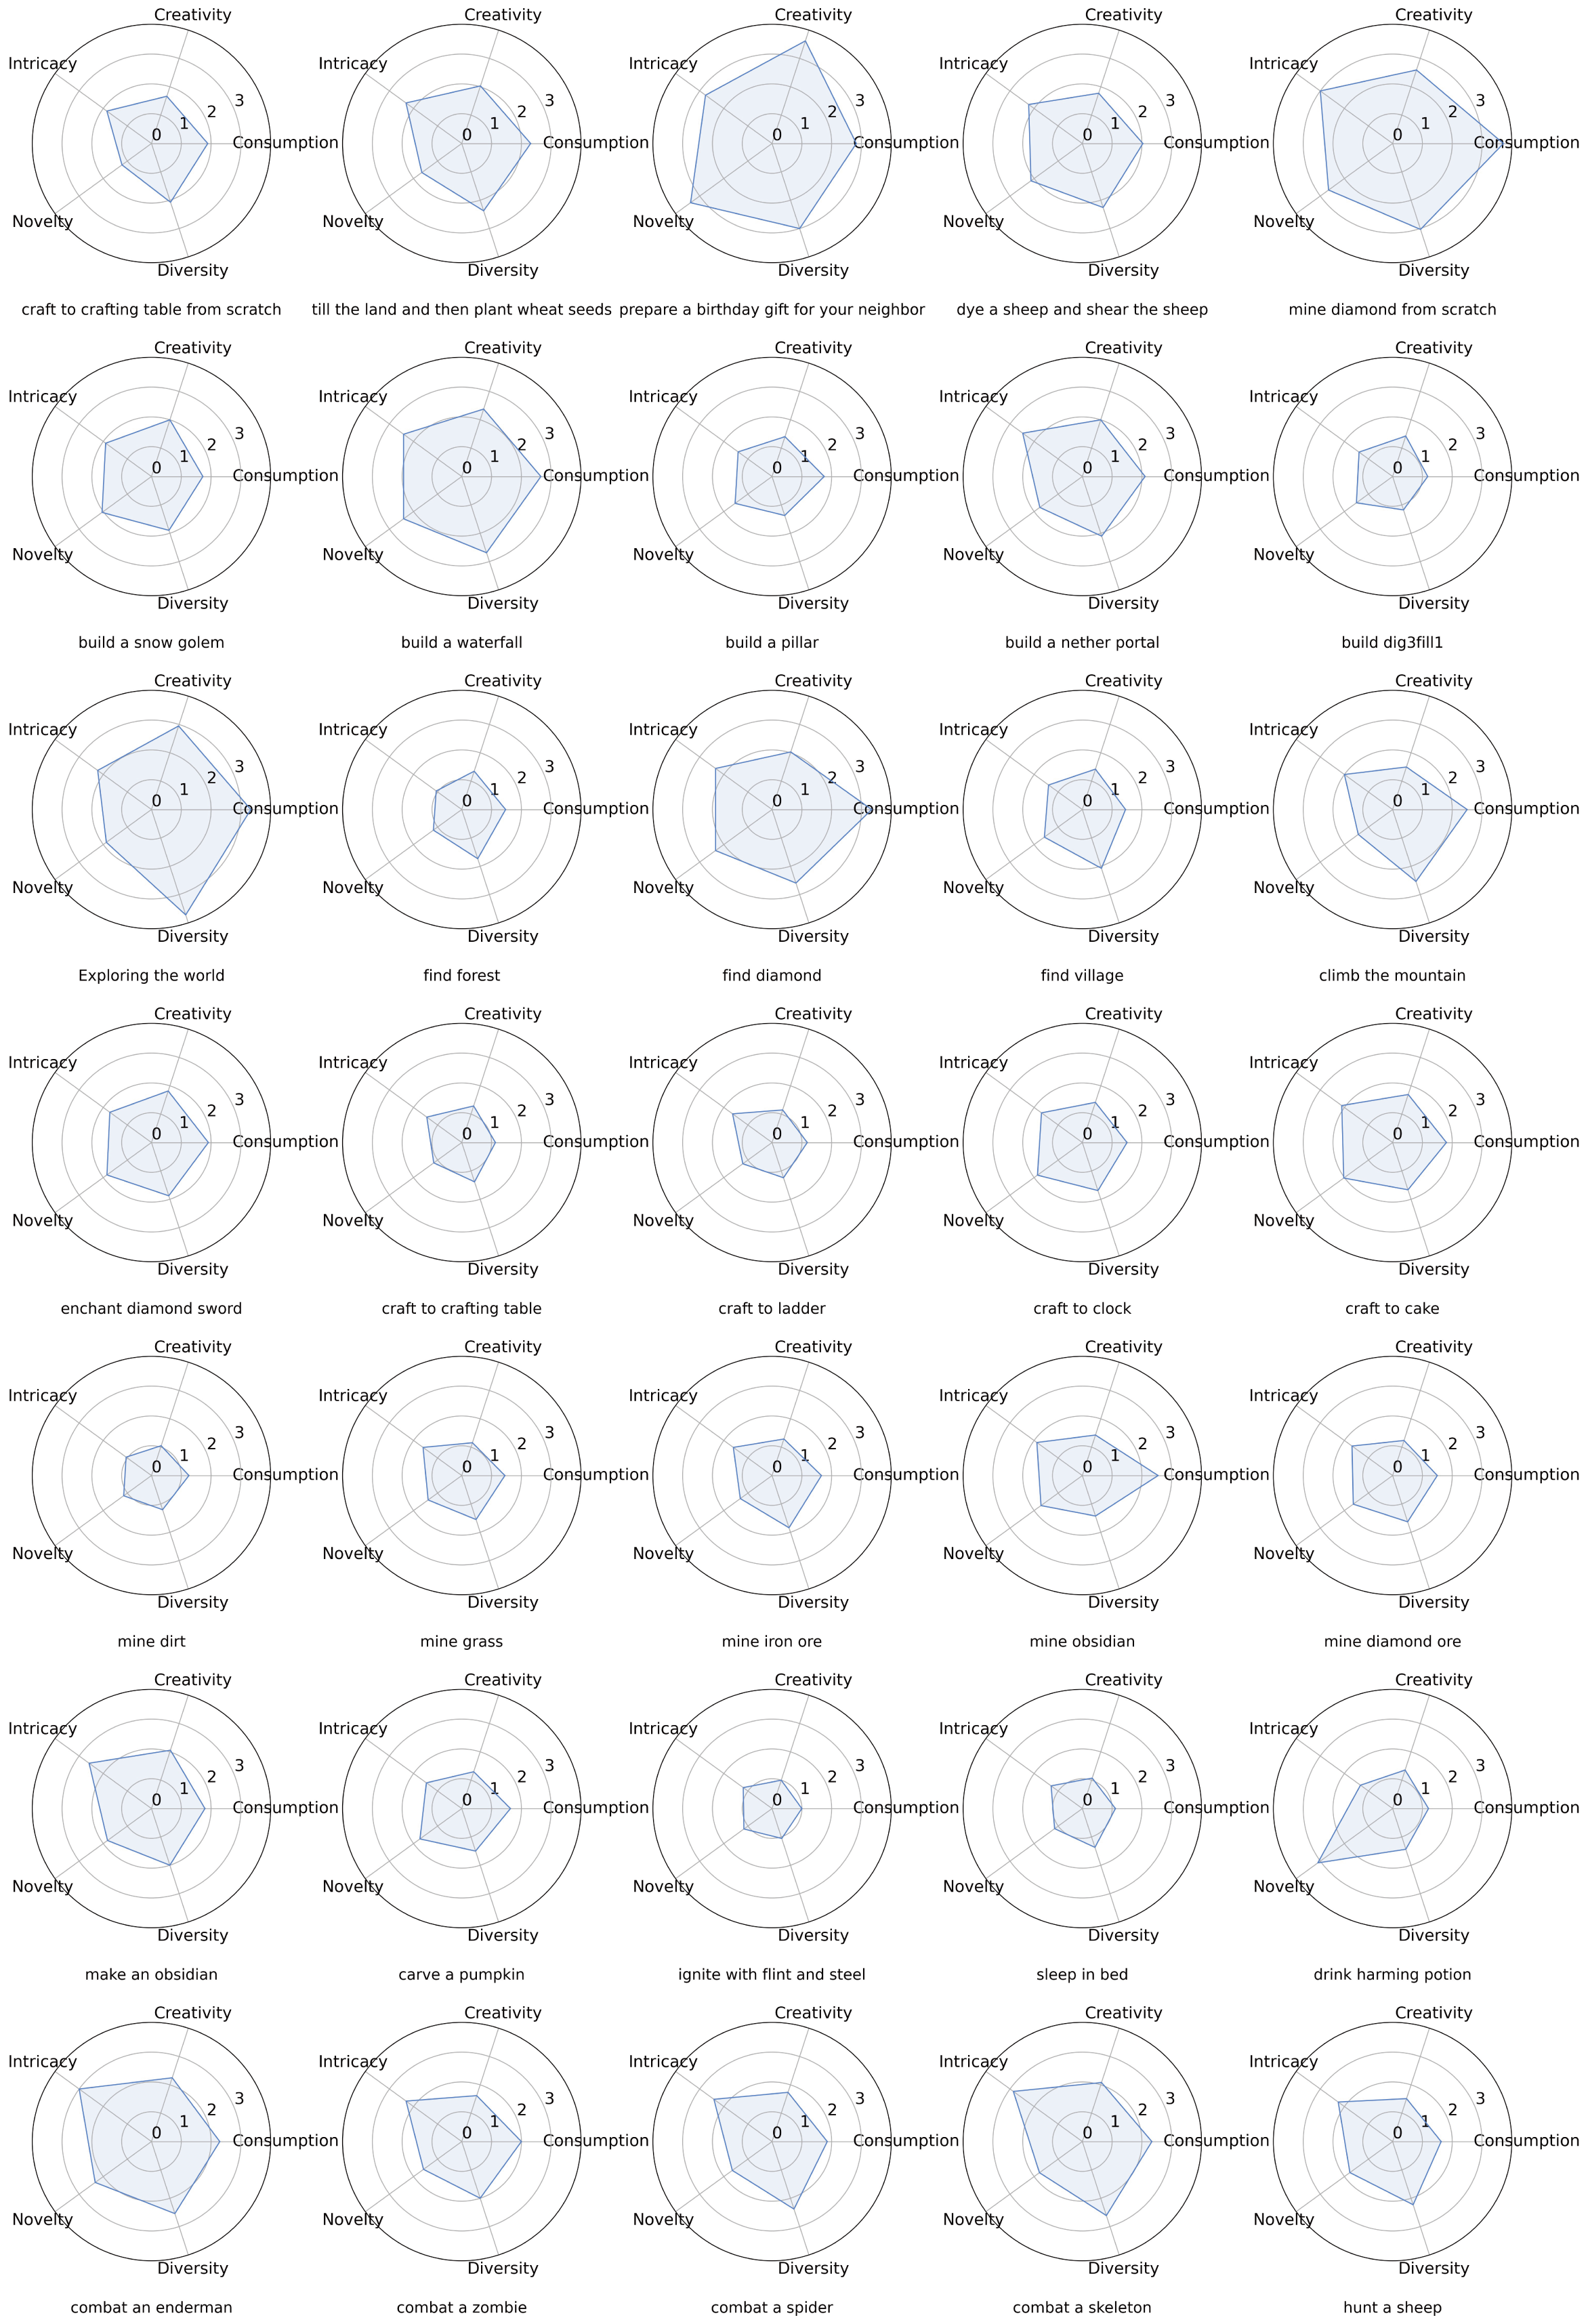
\includegraphics[width=0.9\textwidth]{figs/difficulty.png}
    \caption{The annotated difficulty score for each task.}
    \label{fig:difficulty-full}
\end{figure}



\section{Task Annotation}
\label{app.annotation}
We use stratified sampling for different task groups, making the selection of tasks for each group diverse and representative, and at the same time, focus on the different groups fairly. More precisely, for each task group $r$, our selected task $\mathcal T$ meets 
$$
\mathcal T|r \sim \mathcal P(t|r)
$$ 
and for each task $t$,
$$
S_0|t \sim \mathcal P(s_0|t)
$$
The former represents the representativeness and diversity of tasks in each group, which has been demonstrated by the high entropy of the sampled tasks. Later we will elaborate on how to manipulate our environment configurations to try to make the distribution of $s_0$ conform to the latter formula as much as possible.

In order to compare the performance of the model output with the performance of human players, video data of human players is needed. We will also annotate the videos we recorded.

\fi



\subsection{Human Videos For Tasks}
\label{app:human_video}
Human videos serve two purposes: they are used as reference videos for GROOT and for comparison with the trajectory videos generated by the agent models. For each task, we select three world seeds: 19961103, 20010501, and 12345. For each (task, seed) pair, we manipulate the controllable parameters as described above, resulting in three distinct environment configuration files. For each configuration file, we record a corresponding human video. Additionally, we designate the first configuration file of seed 19961103 as the reference video for GROOT.


\subsection{Human rating system}

In our dataset, there are a total of 60 tasks, each containing 10 rollout trajectories in video format. These videos capture gameplay records from either humans or various agents. 

For the \textbf{absolute rating task}, we randomly select one task and present a corresponding video to human raters, who score it across six predefined dimensions. 

For the \textbf{comparative evaluation task}, we randomly sample two different rollouts from the same task, referred to as \textit{Video A} and \textit{Video B}. These videos may both be from human players, both from agents, or one from a human and the other from an agent. Raters are then asked to compare \textit{Video A} and \textit{Video B} on each dimension to determine which one performs better. 

The human rating interfaces are illustrated in Figure~\ref{fig:compare_web} and Figure~\ref{fig:single_web}. Taking the video comparison website as an example, it is designed to evaluate agent performance by displaying two videos side by side, enabling human raters to directly compare their behaviors within the same task. The interface consists of the following modules:

\begin{enumerate}
    \item \textbf{Task Description Module}: Positioned at the top-right, this module specifies the task to be evaluated (e.g., \textit{Survive Shield: Use a shield to ward off zombies}). It ensures that raters understand the objective before scoring.  

    \item \textbf{Video Display Module}: Two videos are presented side by side, each replaying an agent’s gameplay. This layout allows raters to observe agent behaviors, mistakes, or innovative strategies in real-time.  

    \item \textbf{Scoring Panel}: Located below the videos, this panel enables raters to assess agent performance across six dimensions. For each dimension, raters can indicate which agent performed better, mark a tie, or specify that neither agent took relevant actions.

    \item \textbf{Input and Submission Module}: At the top-center, an input box collects rater identifiers to ensure traceability. A \textit{Submit} button at the bottom sends completed ratings to the database, contributing to the dataset used for benchmarking.  
\end{enumerate} 


\begin{figure}[H]
    \centering
    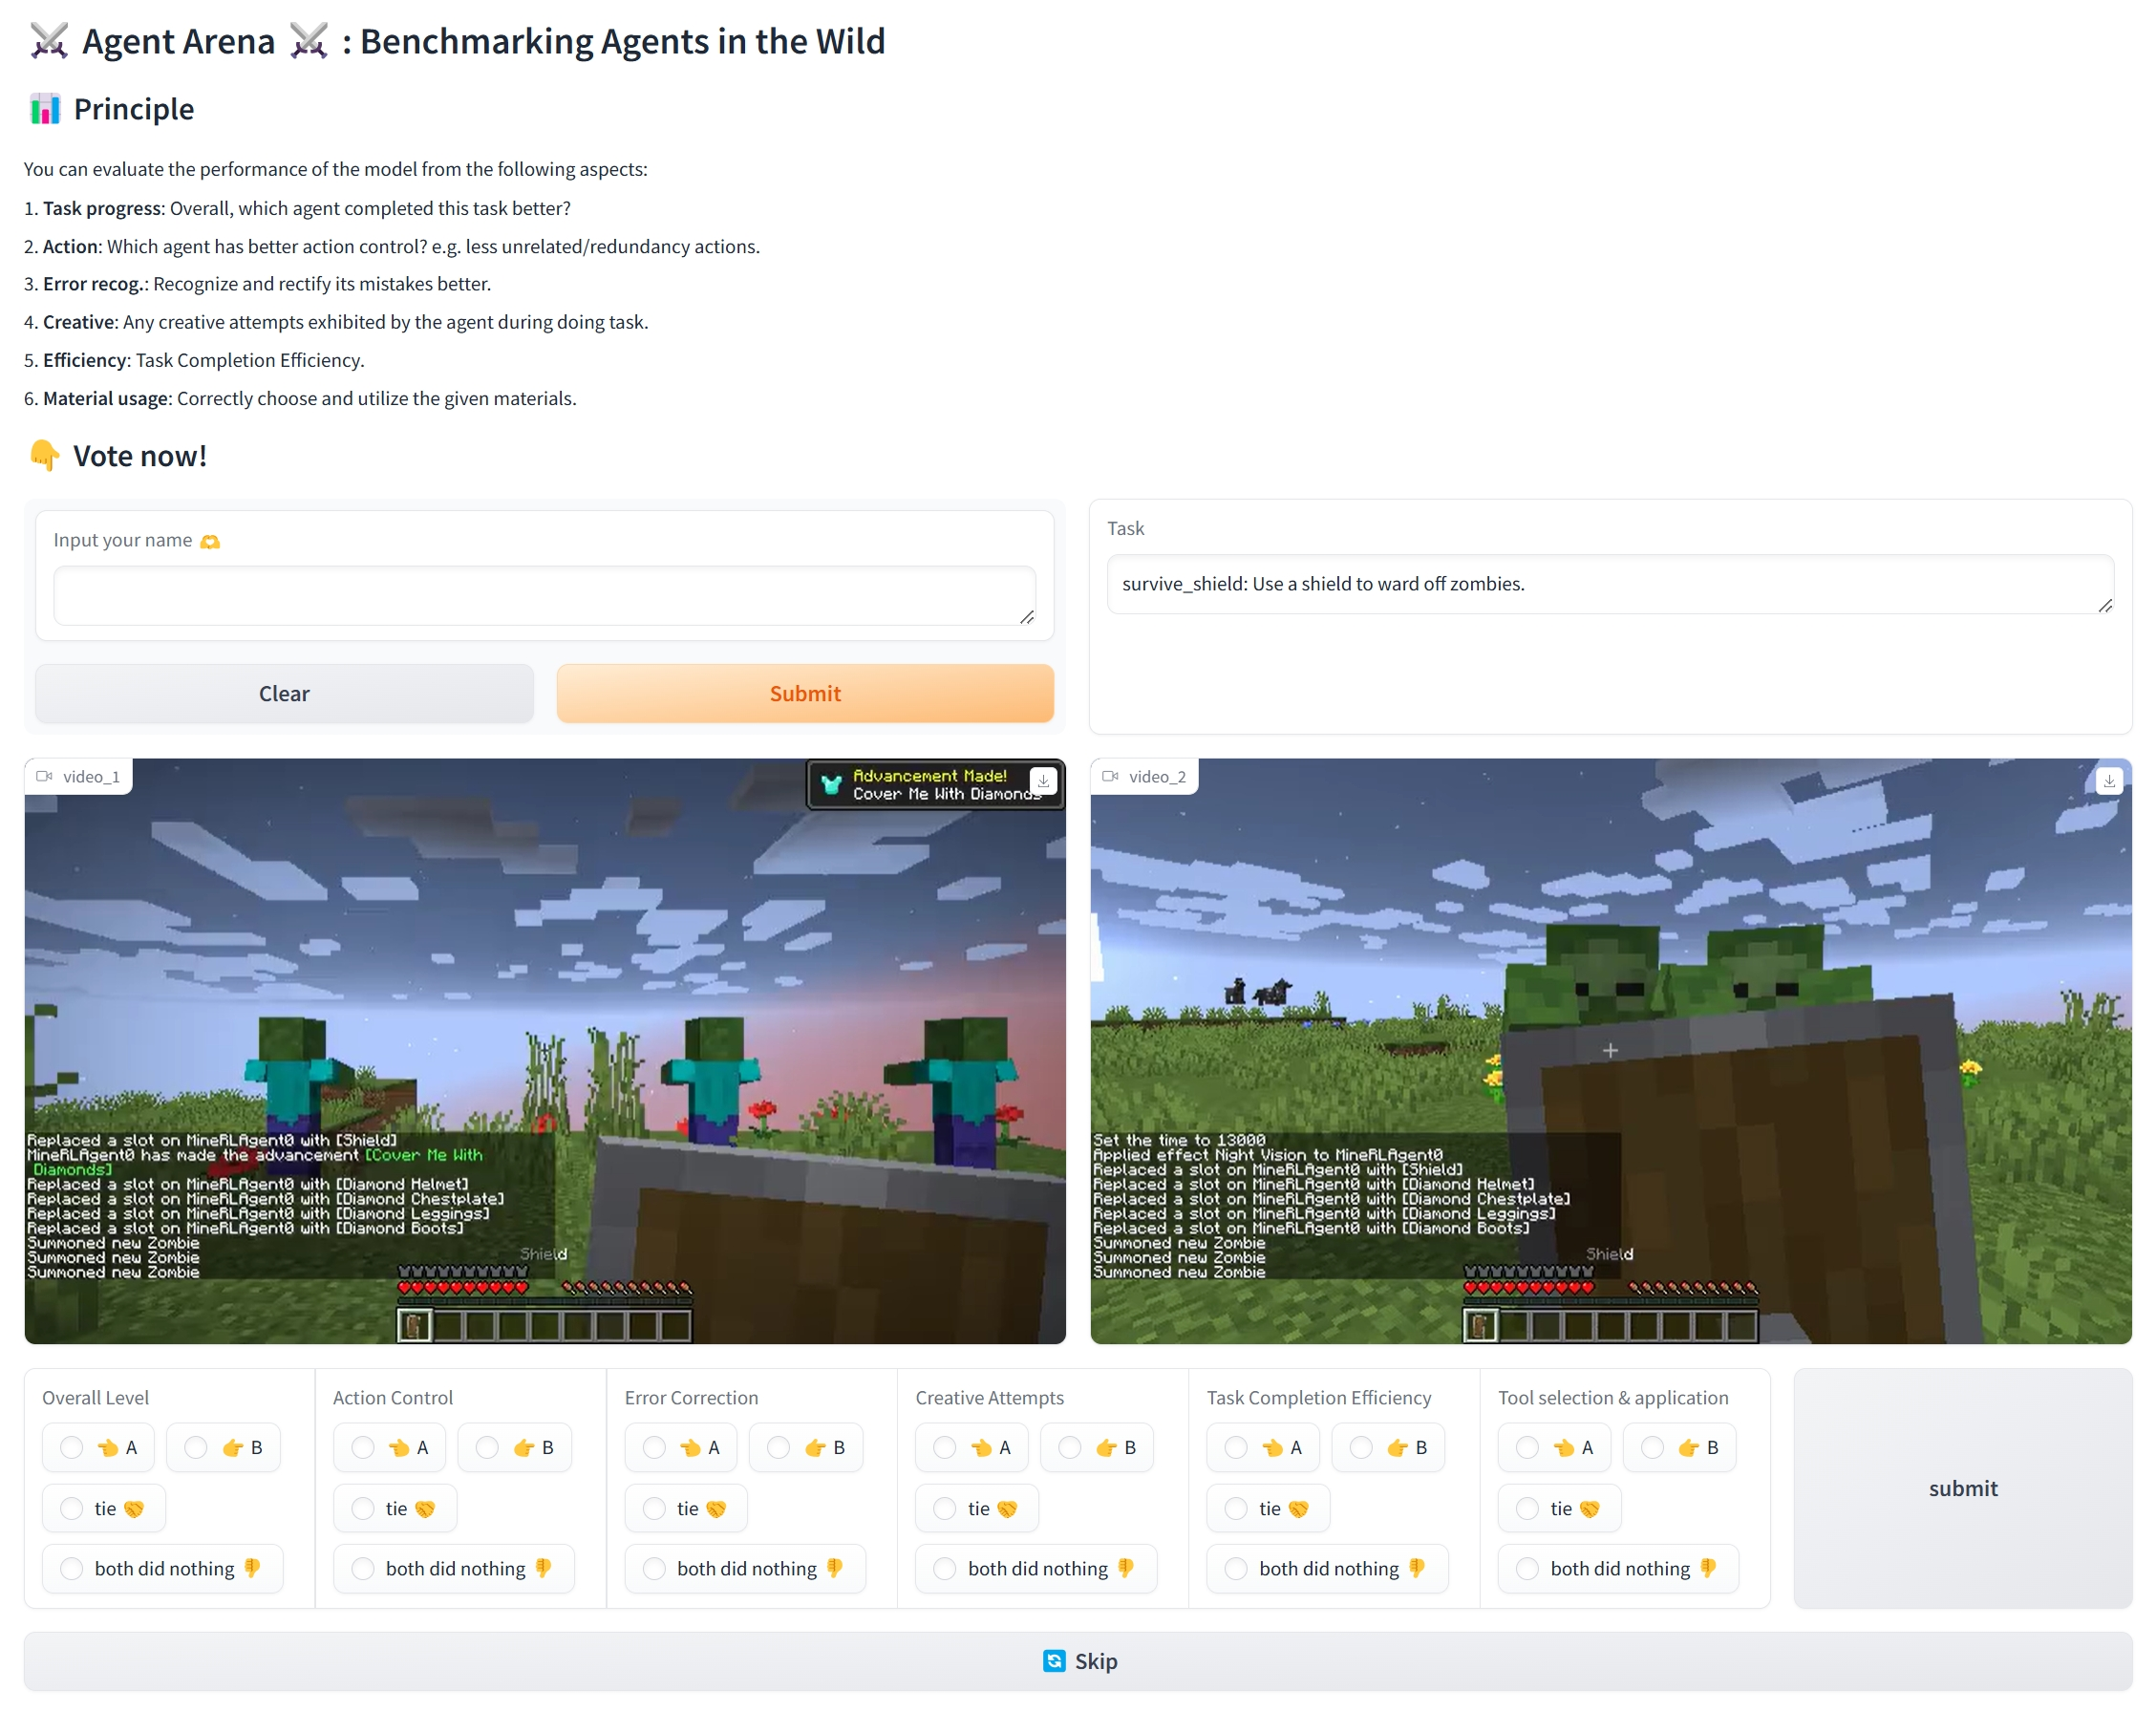
\includegraphics[width=\linewidth]{figs/compare_html.png}
        \caption{Video comparison website.}
        \label{fig:compare_web}
\end{figure}

\begin{figure}[H]
    \centering
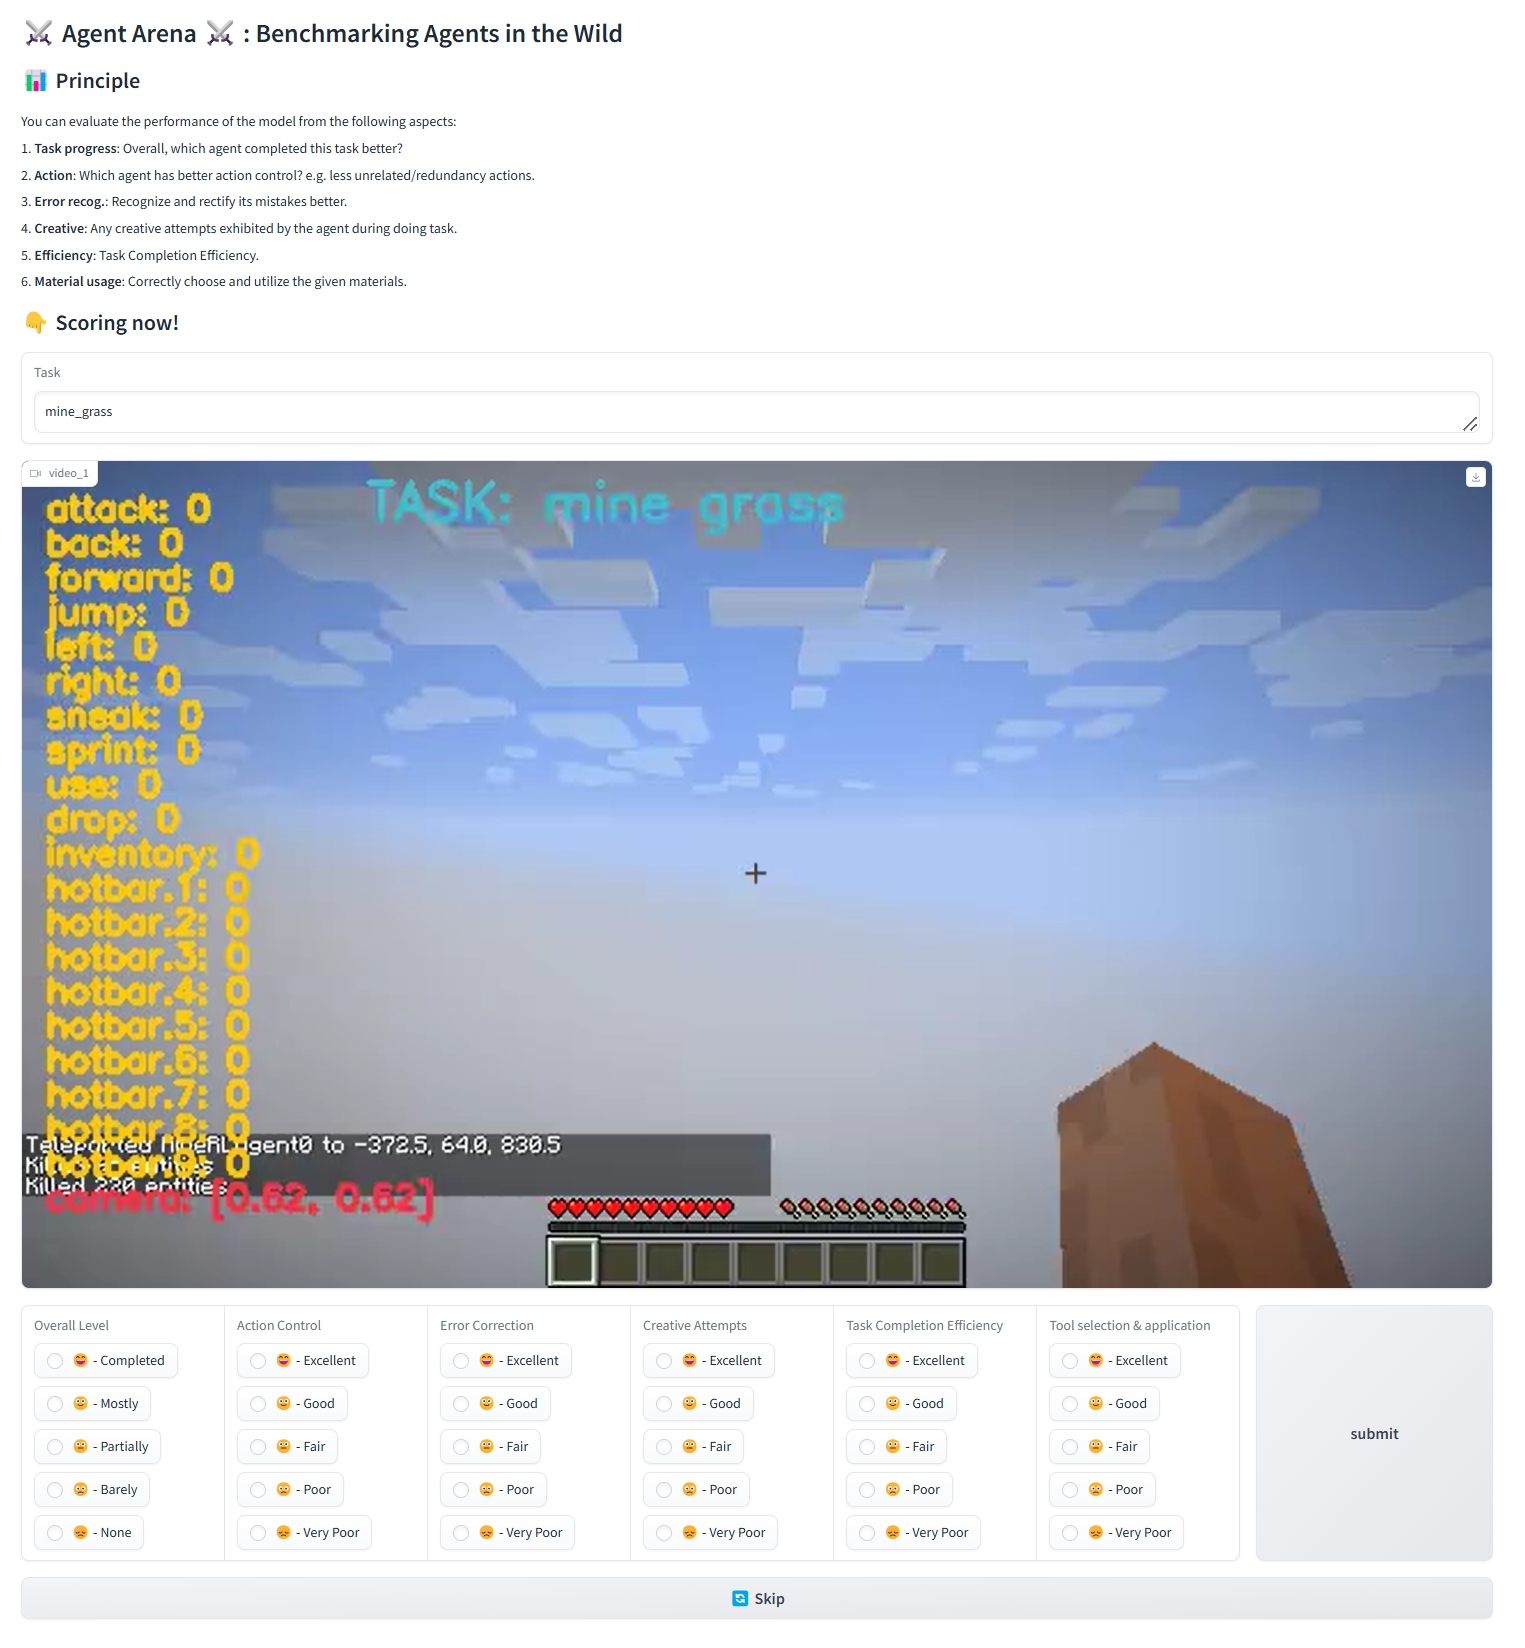
\includegraphics[width=\linewidth]{figs/single_rating_html.png}
    \caption{Individual video rating website.}
    \label{fig:single_web}
\end{figure}












% 

\iffalse
\section{Programmatic Metrics for Studied Tasks}
\label{app.progmetric}
\paragraph{Metrics} During our evaluation, we use the scripts to record information for each video, including items that are crafted, used, broken, and mined, blocks that are mined, entities that are killed, and horizontal and vertical offset. With the scripts, some tasks can be evaluated using programmatic metrics in a fully automated manner, thus saving time and human resources. Table~\ref{tab:task_relationship} shows examples of tasks in our experiments and their corresponding metrics. The threshold for the task 'Explore the world' is 50 units, while for the task 'Climb the mountain,' it is 20 units in seed1 and 30 units in seed2.

\paragraph{TrueSkill Rating} We also evaluate and compare the previous agents through the TrueSkill rating system. It was developed by Microsoft Research and is currently used in matchmaking and ranking services on Xbox LIVE. It takes the uncertainty of the players' ability into consideration and models the score of a player as a Gaussian distribution $\mathcal N(\mu, \sigma^2)$, then uses the Bayesian inference algorithm to measure a player’s score, where $\mu$ is the average skill of the player and $\sigma$ is the standard deviation of a play's performance. A real skill of the player is between $\mu \pm 2\sigma$ with $95\%$ confidence. The result of TrueSkill Rating is shown in Figure~\ref{fig:trueskill_in_group}.


\begin{table}[h]
  \centering
  \resizebox{0.99\linewidth}{!}{
  \begin{tabular}{c|c}
    \hline
    {\multirow{2}{*}{\textbf{Task}}} & {\multirow{2}{*}{\textbf{Metric}}}\\
    &\\
    \hline
    Build snow golem 
    &Success rate
    \\
    Build pillar
    &Success rate to build a pillar at with least 5 blocks
    \\
    Build dig3fill1
    &Success rate
    \\
    Build nether portal
    &Success rate
    \\
    Build a waterfall
    &Success rate
    \\
    
    Craft to ladder
    &Success rate
    \\
    Craft to crafting table
    &Success rate
    \\
    Craft to clock
    &Success rate
    \\
    Craft to cake
    &Success rate
    \\
    Enchant diamond sword
    &Success rate
    \\
    Combat zombies
    &Success rate
    \\
    Combat spiders
    &Success rate
    \\
    Combat skeletons
    &Success rate
    \\
    Combat enderman
    &Success rate
    \\
    Hunt a sheep
    &Success rate
    \\
    
    \multirow{2}{*}{Mine grass}
    &Success rate when the number of grass blocks and tall grass blocks\\
     & mined in total exceeds the threshold.
    \\
    Mine obsidian
    &Success rate 
    \\
    Mine dirt
    &Number
    \\
    Mine diamond ore
    &Success rate
    \\
    Mine iron ore
    &Success rate
    \\
    Explore the world
    &Success rate when the horizontal offset is greater than the threshold.
    \\
    Find a forest
    &Success rate to stay in forest for last 10s
    \\
    Find a village
    &Success rate to stat to village for last 10s
    \\
    Find diamond
    &Success rate
    \\
    Climb the mountain
    &Success rate when the height offset is greater than the threshold.
    \\
    Drink harming potion
    &Success rate
    \\
    Carve pumpkin
    &Success rate
    \\
    Make fire with flint and steel
    &Success rate
    \\
    Make obsidian by water
    &Success rate
    \\
    Sleep in bed
    &Success rate
    \\

    
    Dye a sheep and then shear the sheep
    &Success rate
    \\
    Mine diamond from scratch
    &Success rate
    \\
     Craft to crafting table from scratch
    &Success rate
    \\
    Till the land and then plant wheat seeds
    &Success rate
    \\



    \hline
  \end{tabular}
  }
  \caption{The programmatic metric for each task.}
  \label{tab:task_relationship}
\end{table}





\begin{figure}[h]
    \centering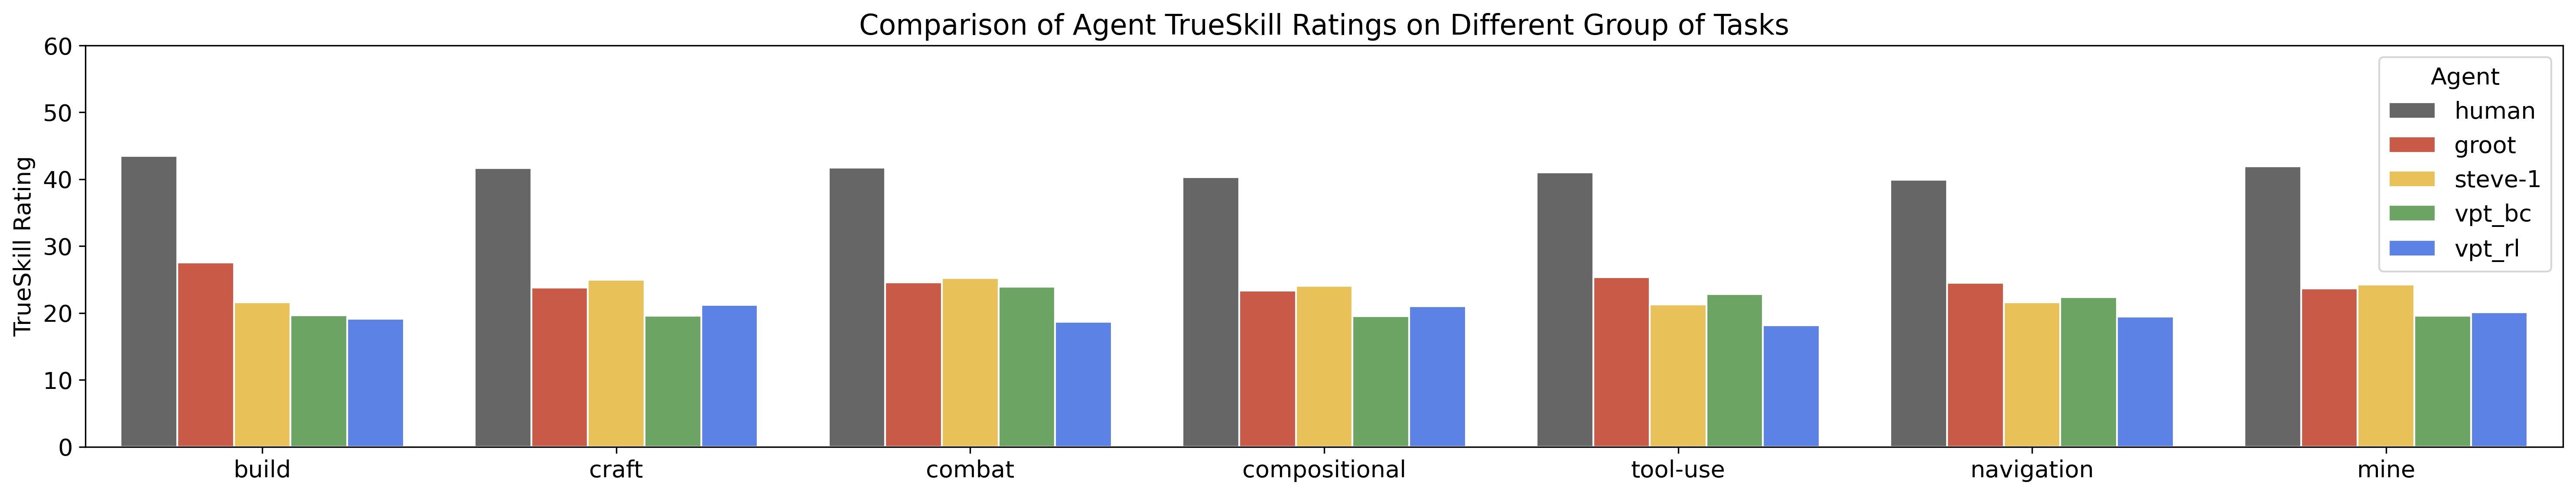
\includegraphics[width=0.9\linewidth]{figs/true_skill_in_group.png}
    \caption{Comparison of Agent TrueSkill Ratings on Different Groups of Tasks}
    \label{fig:trueskill_in_group}
\end{figure}



\section{Minecraft Environment Simplification in Previous Works}
\label{app.simplification}
In our evaluation mechanism, we require the agent's observation space and action space similar to a human player playing in front of a device. In other words, all the information that needs to be perceived comes from the pixels displayed on the screen, and the underlying control relies on simulating mouse and keyboard operations. The only difference is that the degree of freedom is slightly lower, that is, the keyboard operations only allow the types shown in~\Cref{tab:actionspace}.  However, in order to develop a Minecraft agent more efficiently, some previous works did not meet these requirements. Some benchmarks simplified the observation space and action space, and some previous agents further simplified the benchmarks. Some of them reduced the freedom of operation by changing the action space, others utilized some additional information within the game that cannot be obtained from the pixels.

\subsection{Prevoius Benchmarks}

\paragraph{MineRL} MineRL~\citep{minerl} is a benchmark for Minecraft agent competition, and there are different unrelated tasks to evaluate. Before version 0.4.4, MineRL offered different action spaces and observation spaces for each task, and for each task, the spaces are exactly what is needed to complete this track. After version 1.0.0, the observation space is the same as in this paper, and the action space is similar to ours, except for two high-level actions - ``pickItem'' and ``swapHands''.

\paragraph{MineDojo} The observation space of MineDojo~\citep{minedojo} simplifies the environment to a large extent. Apart from the ego-centric RGB frames, it can obtain the 3D voxels, nearby tools, damage sources, and lidar, which are extra in-game information, equipment, inventory, life statistics, GPS location, and compass, which should be derived from the pixels. As for the action space, some high-level actions are encapsulated such as ``craft'' and ``equip''.

\paragraph{BEDD} The observation space of BEDD~\citep{milani2023bedd} is the same as ours. It requires actions to directly simulate mouse and keyboard operations but does not limit whether to encapsulate high-level actions. 


\subsection{Previous Agents}

\paragraph{VPT} VPT~\citep{vpt} does little to simplify the environment. The only difference between VPT and our benchmark is that VPT disables F3 key, but it does not make use of the information in it.

\paragraph{DEPS} The experiment of DEPS contains two parts. Both MineRL and MineDojo benchmarks have been tested and each experiment follows the action space and observation space of the corresponding benchmark.

\paragraph{Voyager} The information used by Voyager~\citep{voyager} is less similar to human players. Voyager runs in a Minecraft world by incrementally building a skill library, which stores action programs, whose code is generated by GPT-4~\citep{gpt4}. The observation of Voyager includes the feedback of GPT-4 and it knows its inventory directly.

\paragraph{GITM} Ghost in the Minecraft~\citet{gitm} The observation space is the same as MineDojo and the action space is also structured. Some actions are very high-level, such as ``explore''.

\paragraph{Steve-1} Steve-1 has the same observation space and action space as VPT.

\paragraph{GROOT} GROOT has the almost same observation space and action space as VPT, except dropping items is not allowed (i.e., the Q key is disabled).



%



\begin{figure}
    \centering
    % \vspace{-1em}
    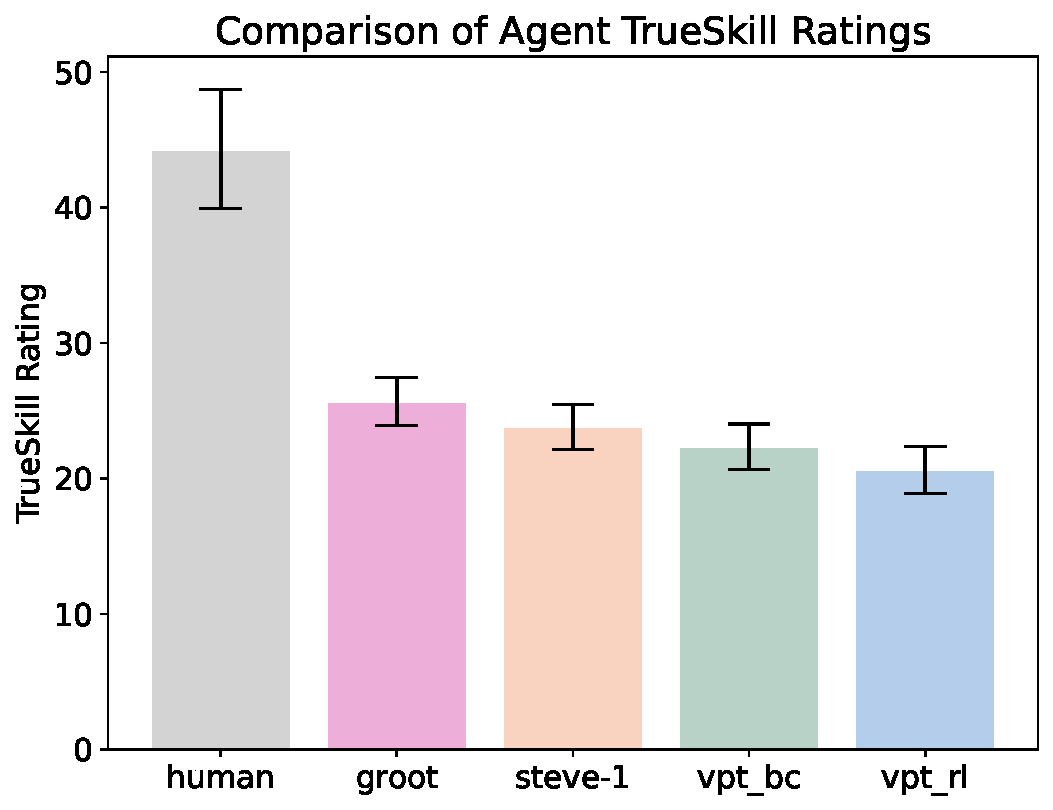
\includegraphics[width=0.4\linewidth]{figs/true_skill.pdf}
    \caption{The TrueSkill evaluation results for the compared agents and human.}
    % \vspace{-3pt}
    \label{fig:true-skill}
\end{figure}


\newpage



\fi


\newpage

\section{Generalization Experiments}
\label{state_space}

In this experiment, we aim to demonstrate that developing open-ended agents requires selecting an environment with a vast state space. We seek to show that when the state space is limited, learning within such an environment is prone to overfitting rather than fostering genuine skill acquisition. Consequently, when tested in open-ended environments (i.e., the test set prepared for this experiment), the agent is likely to fail in handling unseen scenarios.

\begin{table}[H]
\centering
\caption{Training Hyperparameters}
\resizebox{0.6\linewidth}{!}{
\begin{tabular}{ll@{\hskip 2cm}ll}
\toprule
\textbf{Hyperparameter} & \textbf{Value} & \textbf{Hyperparameter} & \textbf{Value} \\ 
\midrule
Steps & 25M & GAE Lambda & 0.95 \\ 
Learning Rate & $2 \times 10^{-5}$ & PPO Clip & 0.1 \\ 
Scheduler & Linear & Policy Loss Weight & 1.0 \\ 
Optimizer & Adam & Value Loss Weight & 0.5 \\ 
Adam Epsilon & $1 \times 10^{-8}$ & KL Loss Weight & 0.3 \\ 
Number of Training GPUs & 2 & KL Loss Decay & 0.995 \\ 
Batch Size per GPU & 1 & Reward Discount & 0.999 \\ 
\bottomrule
\end{tabular}
}
\label{tab:hyper}
\end{table}

\begin{figure}[H]
    \centering
    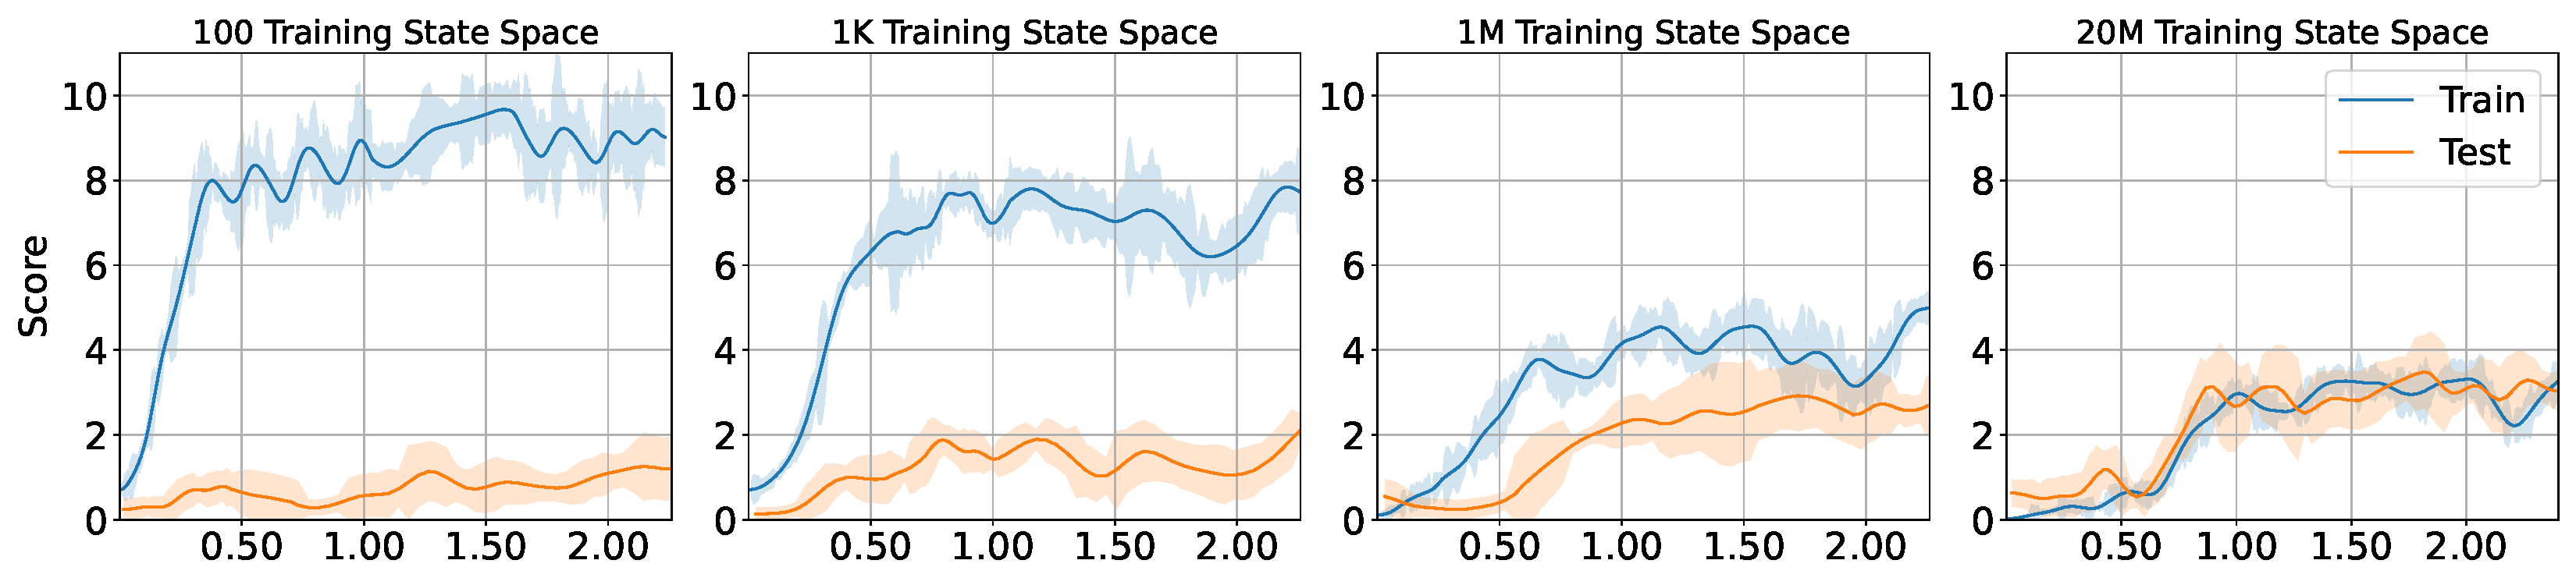
\includegraphics[width=1.0\linewidth]{figs/increase_state.pdf}
    \caption{Generalization performance across different training state sizes. The x-axis values should be multiplied by $10^7$. We evaluate the agent on the full distribution of state space. The mean and standard deviation are computed over 100 episodes. As the number of training states increases, the gap between training and testing performance narrows: training curves become lower, while testing performance improves.}
    \label{fig:increase_state}
\end{figure}

\subsection{Experimental Setup} 
To assess the impact of state space size on generalization, we conduct experiments on the \emph{Hunt Sheep} task, using training sets ranging from $100$ to $10,000,000$ states. The state space primarily consists of variables such as equipment, mobs, biome, distance, and the number of sheep. For each setting, a subset of the state space is sampled as the training set, while evaluation is performed on the full state space. 

We train agents using online reinforcement learning with Proximal Policy Optimization (PPO) for 25 million steps, requiring approximately 50 training hours on three GPUs. Detailed hyperparameter configurations are listed in Table~\ref{tab:hyper}. The implementation is also supported by Minestudio.

\subsection{Results}
As shown in Figure~\ref{fig:increase_state}, agents exhibit strong overfitting when trained on small datasets. As the training set size increases, the generalization gap progressively narrows, with test performance improving as agents become more adept at generalization. To close the generalization gap, agents require exposure to as many as 10 million states.

However, we also observe certain limitations in the agent’s capacity. For example, at the start of the game, sheep may spawn behind the agent, outside its field of view. The agent fails to develop the behavior of scanning its surroundings before proceeding, often becoming distracted by other objects instead.

\subsection{Discussion}
These results highlight the necessity of complex environments like Minecraft, where achieving high performance in a limited state space does not necessarily imply strong generalization. Moreover, sufficiently large state spaces challenge existing reinforcement learning algorithms, offering insights into their capacity limits. At a critical state-space size, further increasing the diversity of states ceases to yield additional improvements in test performance, suggesting an upper bound on the agent’s generalization ability.


\newpage


\section{Large-Scale Inference and Evaluation of MCU}
\label{app:batch_inference}

This section demonstrates the MCU's capability for large-scale inference and task evaluation. We conduct an extensive experiment involving 150 tasks, consisting of 90 atomic tasks and 60 composite tasks. The experiments are performed on three agents: VPT (BC), VPT (RL), and STEVE-1. Due to the high cost of recording reference videos, GROOT is excluded from this evaluation. Specifically, atomic tasks are conducted in \emph{hard} mode, while composite tasks are executed in \emph{simple} mode.

\subsection{Atomic Tasks Setup}
For atomic tasks, one task is randomly sampled from the atomic task list for each experiment. As outlined in~\cref{sec:task_gen}, each selected task undergoes task configuration generation and verification to ensure the necessary preconditions for execution. This process guarantees that tasks are properly configured and validated before being executed in the experimental environment.

\subsection{Composite Tasks Setup}
\label{app:compose_pipeline}
Following the methodology described in~\cref{sec:task_suite}, we implement a composite task generation pipeline using logical connectors (``AND'' and ``OR'') to combine multiple atomic tasks. Composite tasks are designed in three distinct formats, illustrated by the following examples (note that users can define additional compositions):

\begin{enumerate}
    \item \textbf{Three Atomic Tasks Combined with ``AND'' or ``OR''}
    \begin{itemize}
        \item ``Find smooth red sandstone stairs OR mine yellow banner AND sell yellow dye''
        \item ``Find melon AND mine lodestone OR craft a wooden pickaxe''
    \end{itemize}
    
    \item \textbf{Two Atomic Tasks Combined with ``AND'' or ``OR''}
    \begin{itemize}
        \item ``Find melon AND mine lodestone''
        \item ``Craft a wooden sword OR find a diamond''
    \end{itemize}
    
    \item \textbf{Single Atomic Task with No Initial Tools Provided}
    \begin{itemize}
        \item ``Mine red sandstone from scratch''
        \item ``Craft a stone pickaxe from scratch''
    \end{itemize}
\end{enumerate}

In each case, atomic tasks are randomly sampled from a pool of over 3,000 available tasks. Composite tasks are designed to assess the system's ability to handle complex instructions and execute multiple tasks sequentially or in combination.

\begin{figure}
    \centering
    % \rotatebox{90}{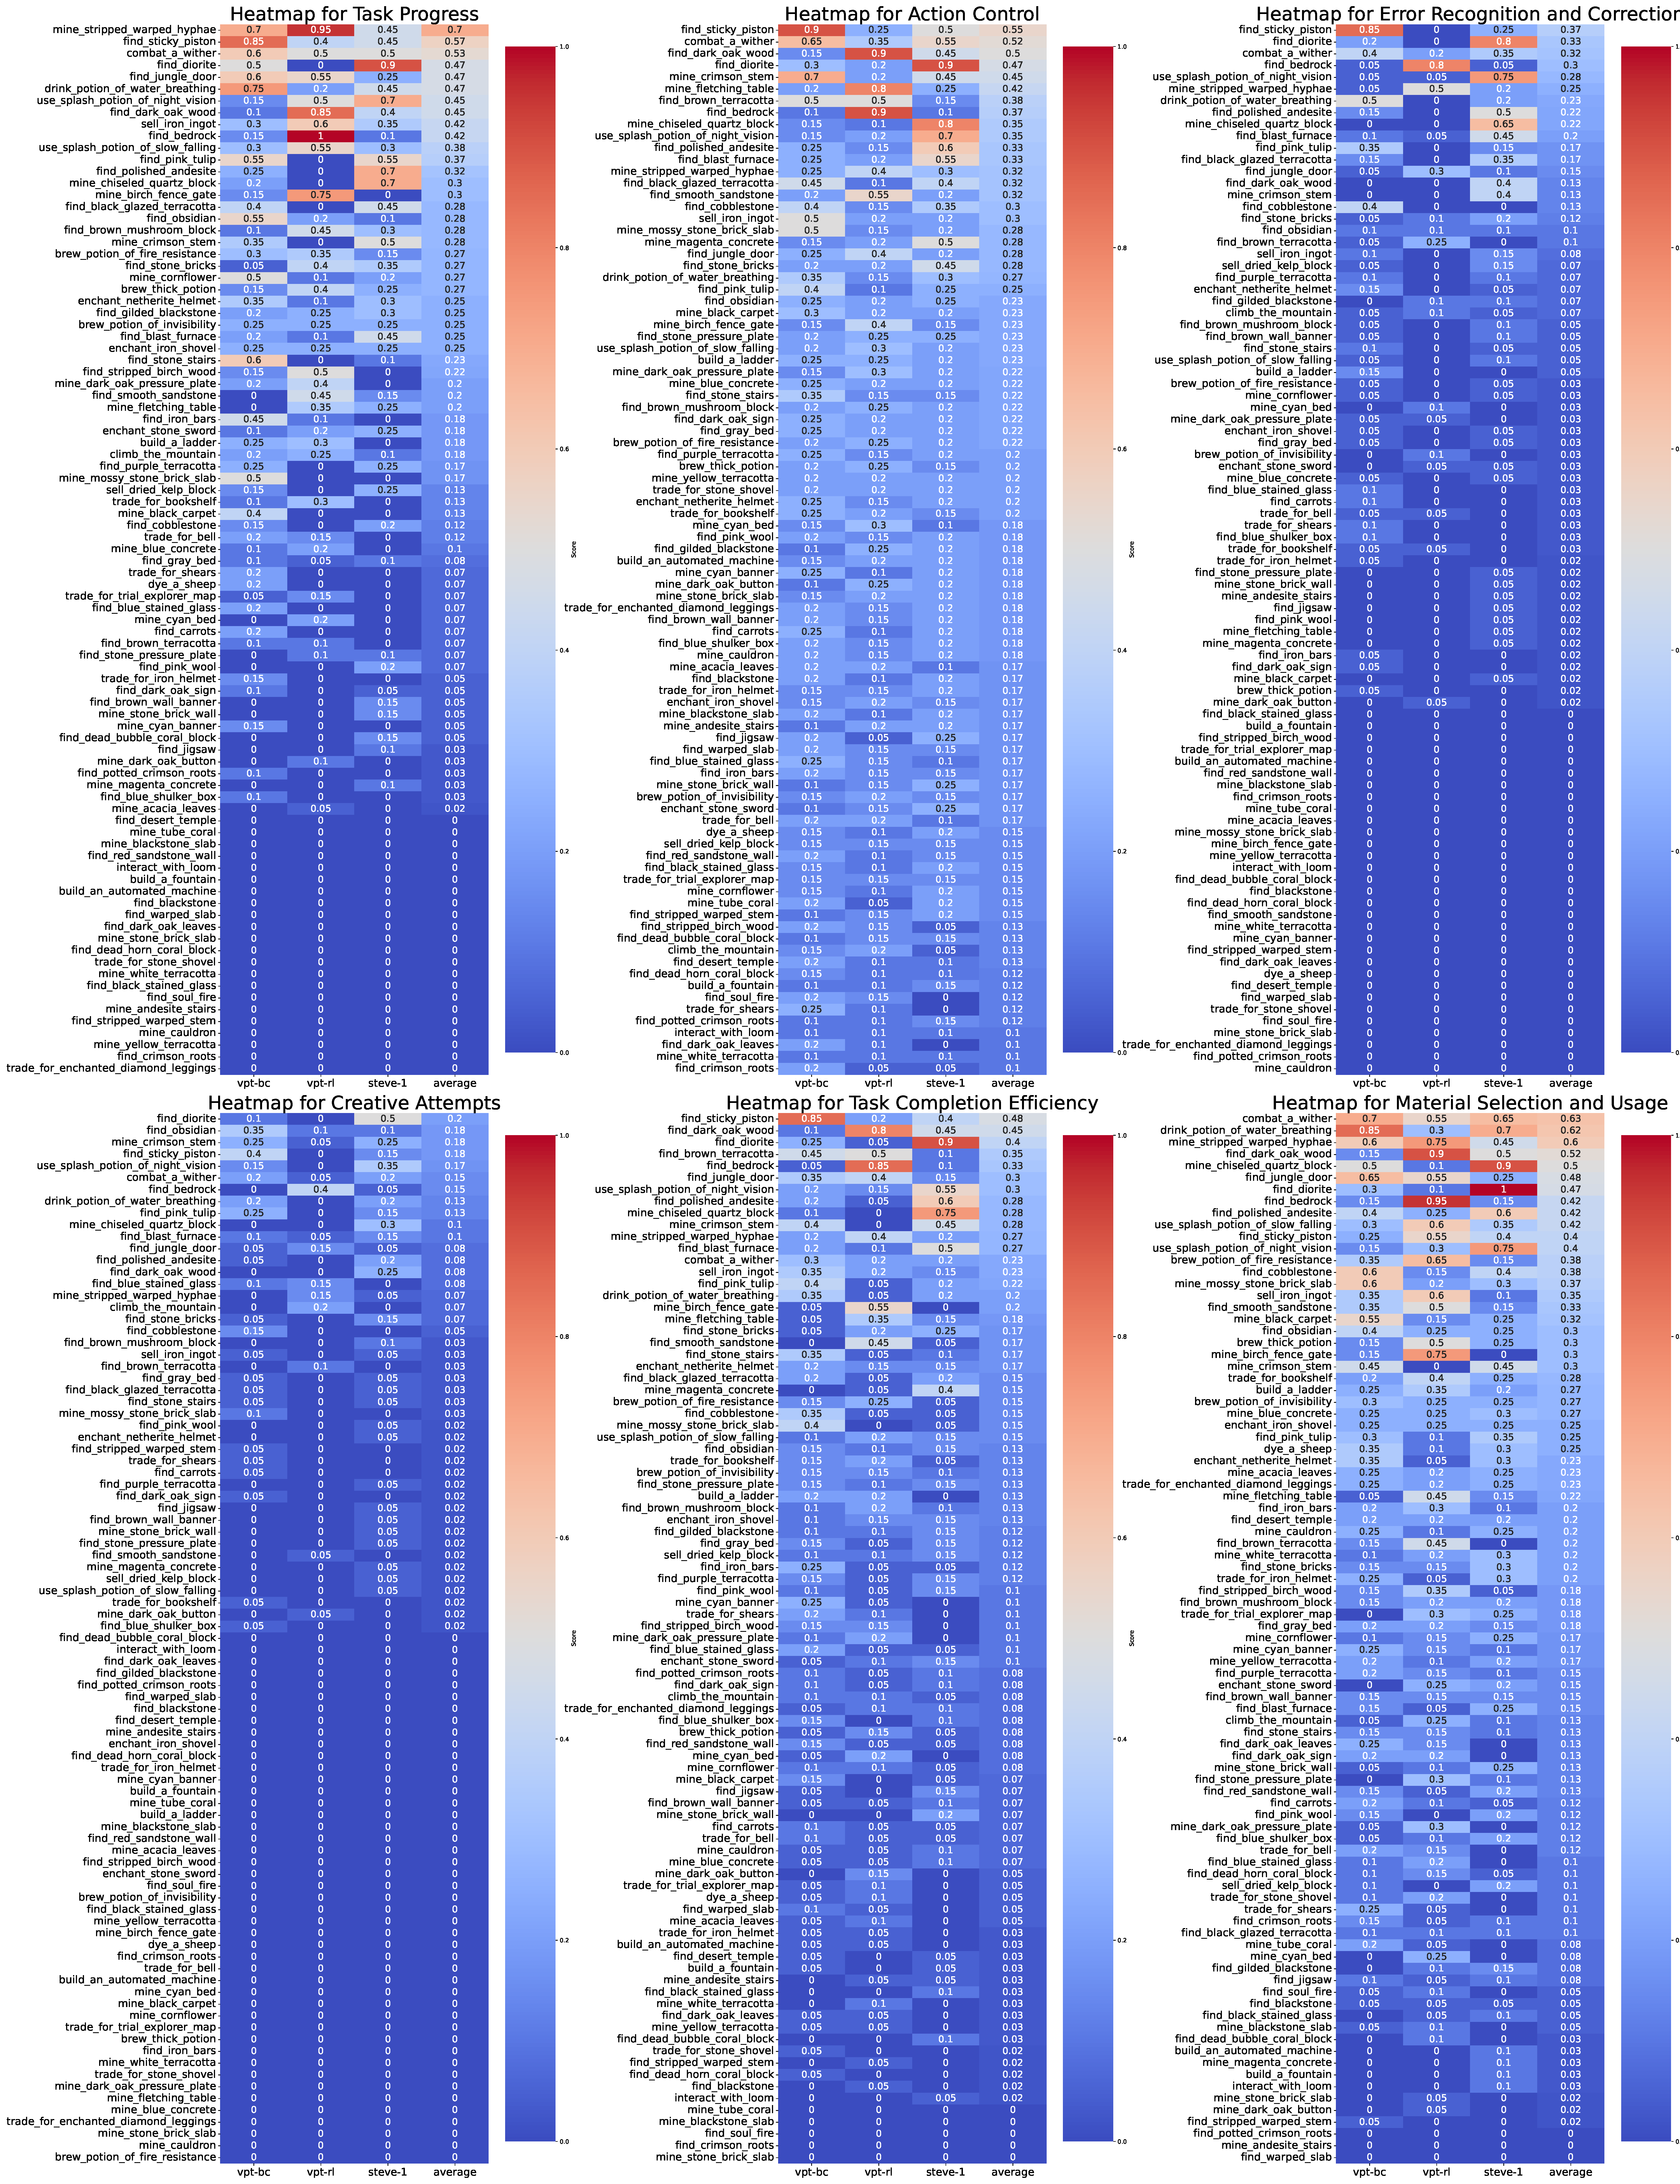
\includegraphics[width=0.9\linewidth]{figs/atomic_app.pdf}}
    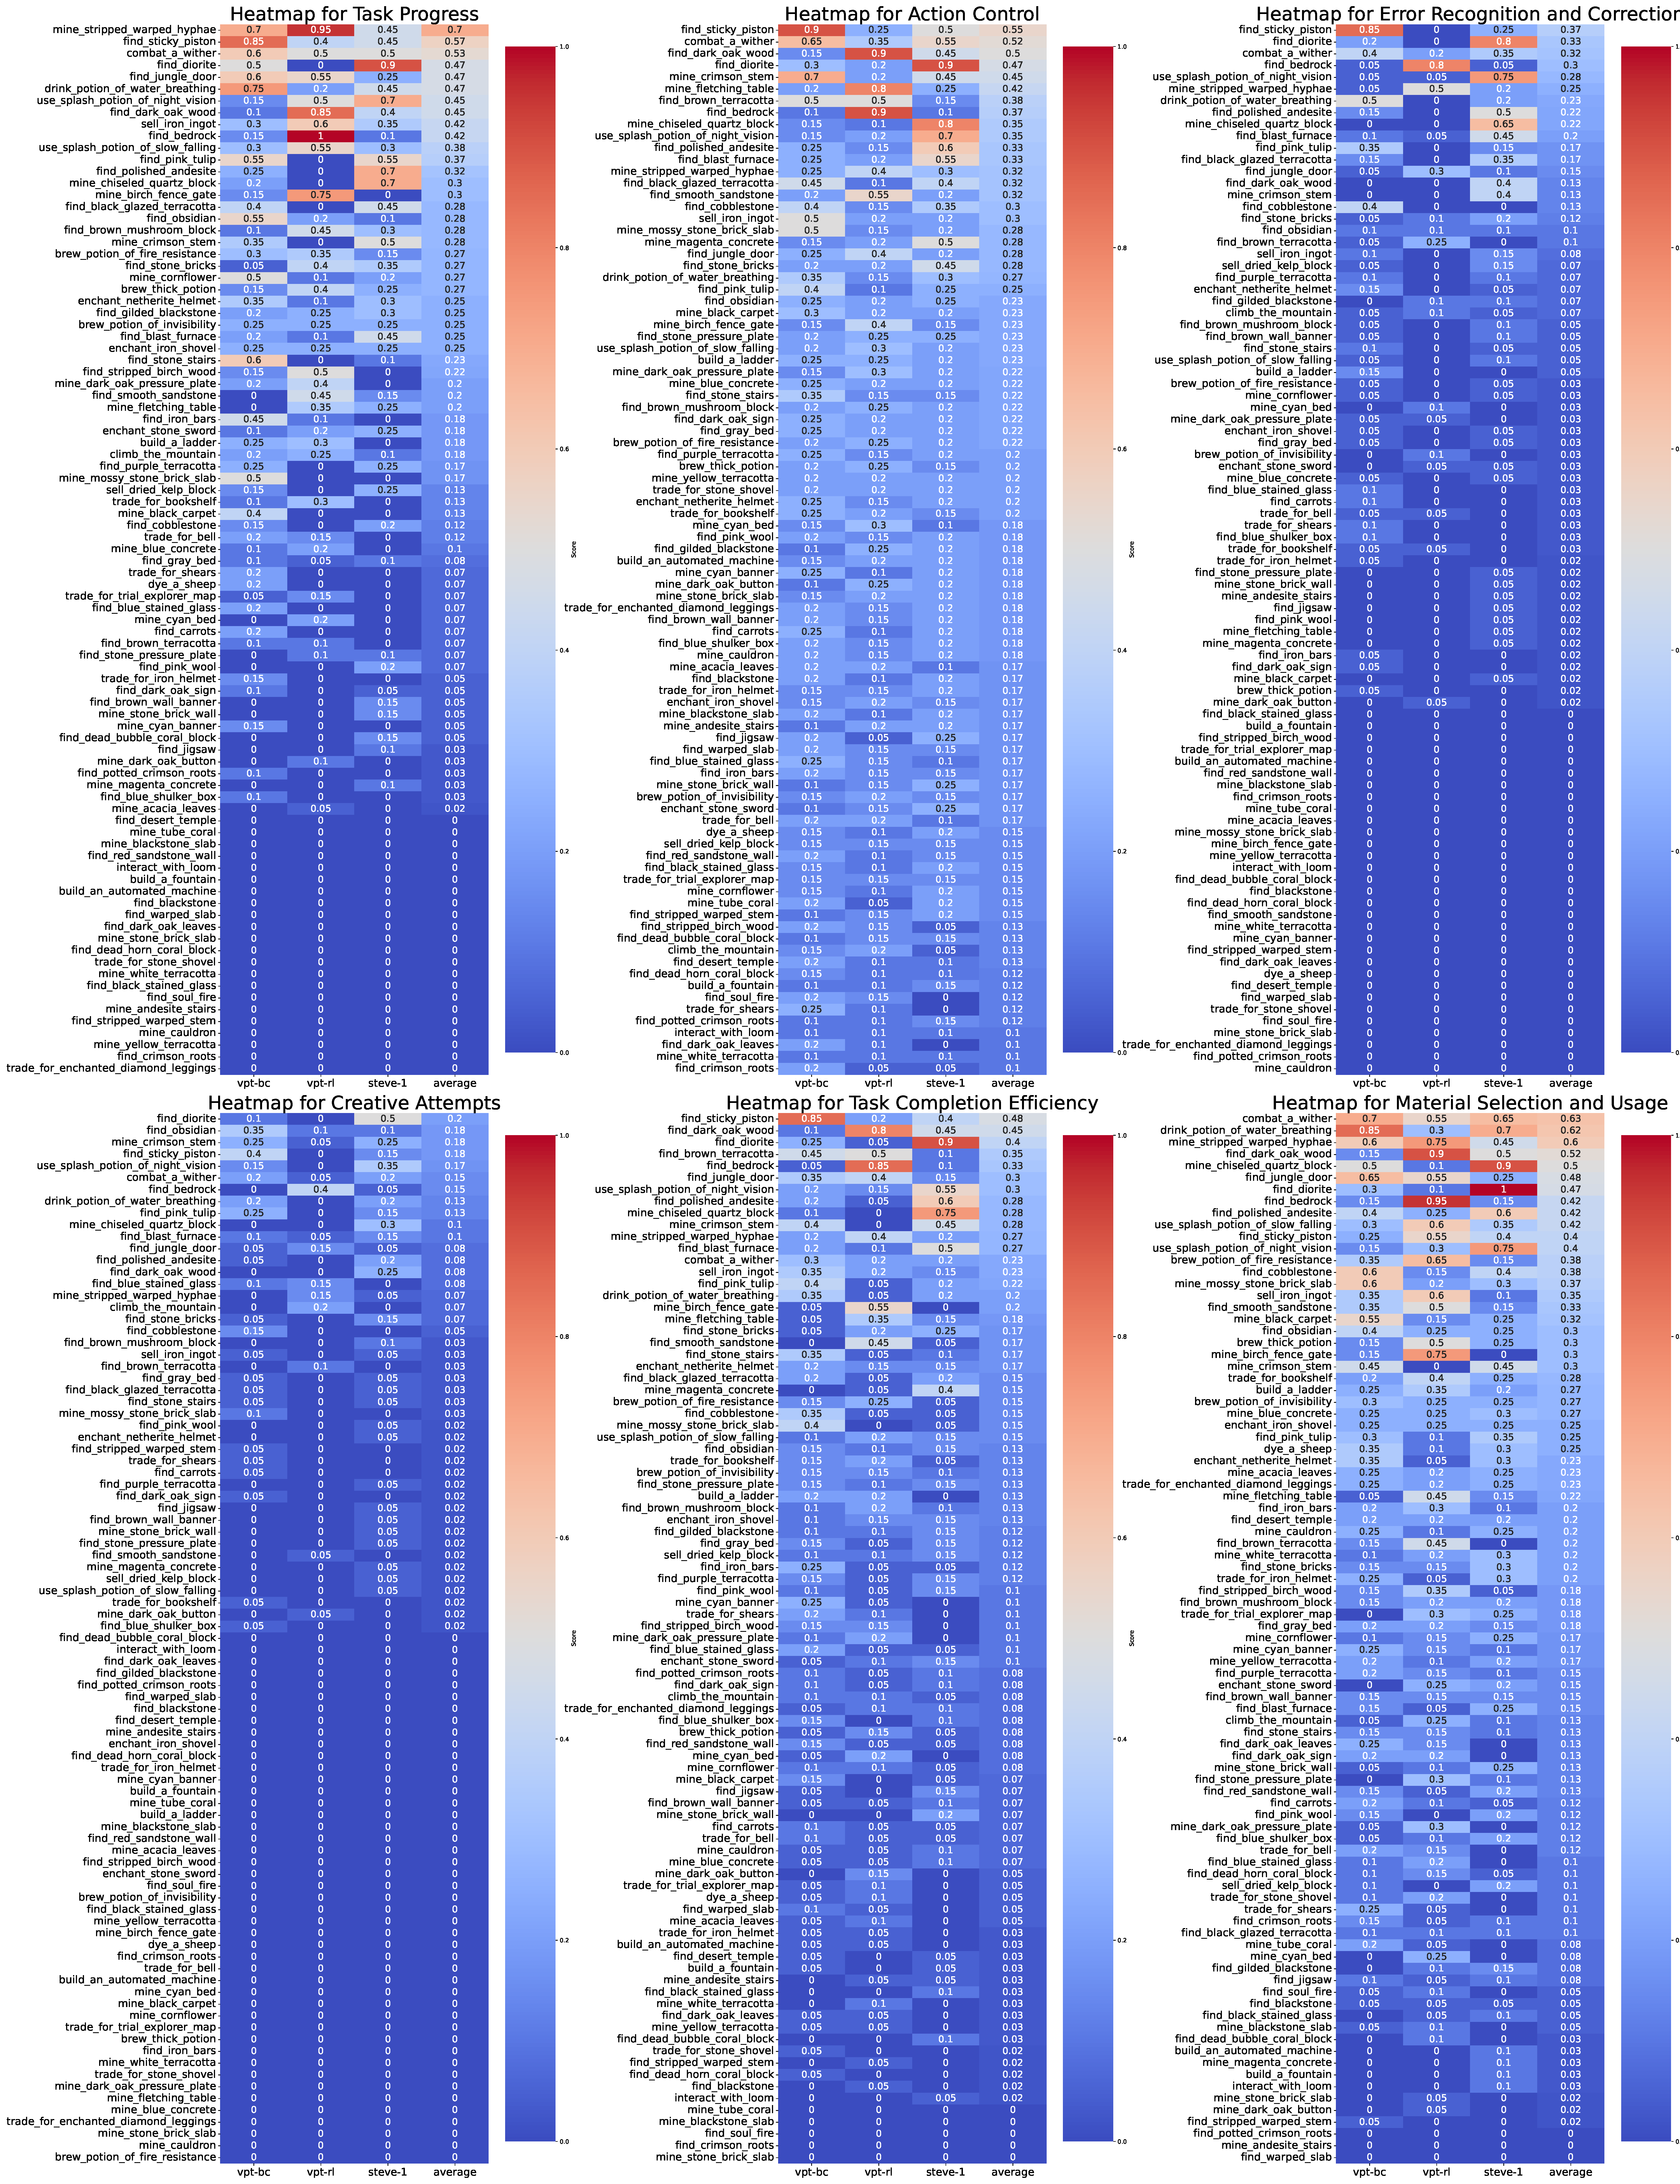
\includegraphics[width=0.95\linewidth]{figs/atomic_app.pdf}
    \caption{Performance of different agents across 90 atomic tasks.}
    \vspace{-3pt}
    \label{fig:atomic_res}
\end{figure}

\begin{figure}
    \centering
    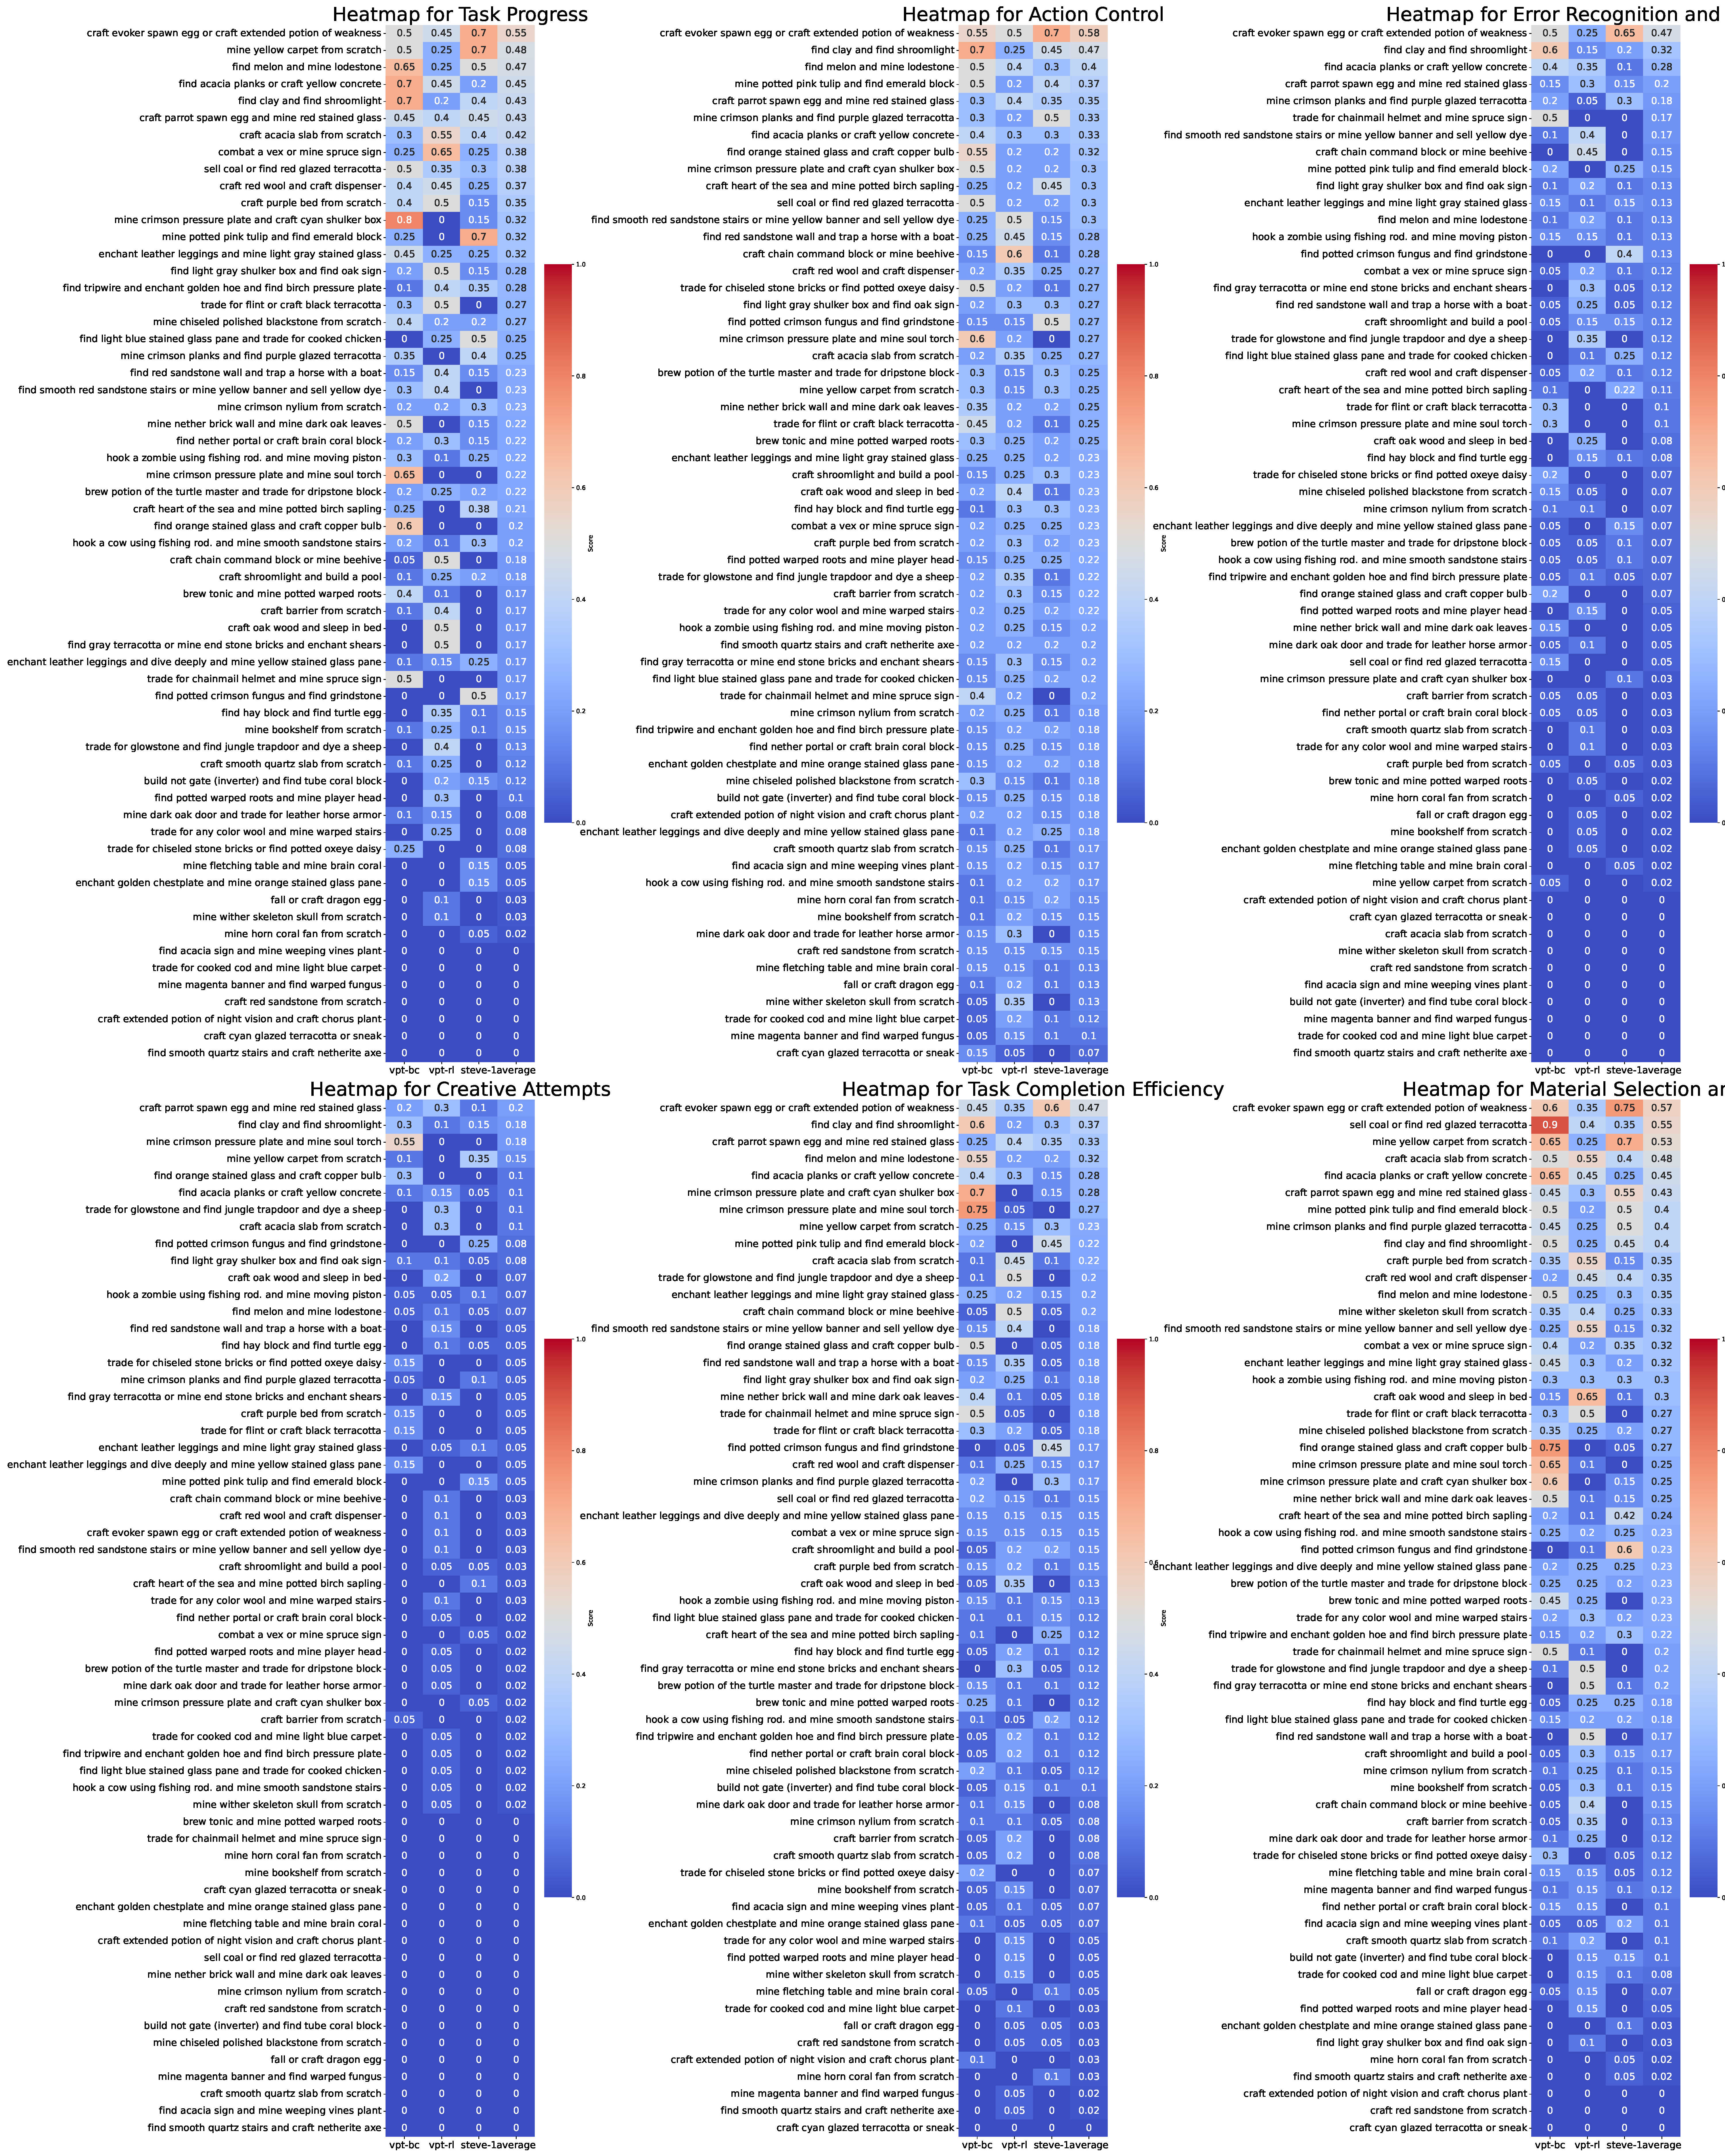
\includegraphics[width=0.99\linewidth]{figs/compose_app.pdf}
    \caption{Performance of different agents across 60 compositional tasks.}
    \vspace{-3pt}
    \label{fig:compose_res}
\end{figure}

\subsection{Experimental Conclusions}
This experiment evaluates agent performance across a broad task domain, focusing on atomic tasks in \emph{hard} mode and compositional tasks. As shown in~\cref{fig:compose_res} and~\cref{fig:atomic_res}, agents struggle with these complex scenarios. STEVE-1 exhibits a performance decline in compositional tasks, likely due to its reliance on short prompts, as discussed in~\citet{steve1}. When encountering longer or unseen instructions, it experiences out-of-distribution (OOD) issues. The low performance of all agents in creativity and error recognition aligns with the conclusions drawn in~\cref{fig:framework}c.




\newpage

\section{MCU-Turbo: A Standard Benchmark for Evaluating Minecraft Agents}
\label{app.mcu-turbo}
We introduce MCU-Turbo, a canonical benchmark suite for systematically evaluating agents within the Minecraft Universal (MCU) framework. MCU-Turbo is designed as a standardized evaluation protocol, comprising 80 atomic tasks across 10 categories and 20 compositional tasks. Each task is assessed under two difficulty regimes—Simple and Hard—to rigorously test an agent’s capabilities in generalization, tool use, long-horizon planning, and robustness to environmental variation. The following experiments establish baseline performance using current state-of-the-art agents.

\subsection{Baseline Results in the Simple Evaluation Mode}
Agents demonstrate varied competencies across different evaluation dimensions under the simple setting. Notably, aspects such as creative behavior and error recognition remain challenging across the board, as illustrated in Table~\ref{tab:baseline_simple}.

\begin{table}[ht]
\centering
\caption{Baseline agent performance in simple mode.}
\label{tab:baseline_simple}
\resizebox{0.99\linewidth}{!}{
\begin{tabular}{lcccccc}
\hline
\textbf{Agent Name} & \textbf{Task Progress} & \textbf{Action Control} & \textbf{Error Recognition} & \textbf{Creative Attempts} & \textbf{Task Efficiency} & \textbf{Material Usage} \\
\hline
STEVE-1 & 31.4\% & 31.9\% & 13.1\% & 6.4\% & 23.2\% & 35.6\% \\
VPT (BC) & 29.1\% & 29.0\% & 11.8\% & 6.2\% & 21.3\% & 33.8\% \\
VPT (RL) & 25.9\% & 26.2\% & 8.8\% & 5.2\% & 18.9\% & 31.3\% \\
JARVIS-VLA & 25.6\% & 27.8\% & 9.3\% & 5.5\% & 18.3\% & 30.5\% \\
\hline
\end{tabular}
}
\end{table}

\subsection{Baseline Results in the Hard Evaluation Mode}
In the Hard mode, agents are subjected to increased environmental complexity and the presence of distractors. As shown in Table~\ref{tab:baseline_hard}, performance consistently declines across all dimensions, underscoring the difficulty of generalization under more challenging conditions.

\begin{table}[ht]
\centering
\caption{Performance degradation in hard mode.}
\label{tab:baseline_hard}
\resizebox{0.99\linewidth}{!}{
\begin{tabular}{lcccccc}
\hline
\textbf{Agent Name} & \textbf{Task Progress} & \textbf{Action Control} & \textbf{Error Recognition} & \textbf{Creative Attempts} & \textbf{Task Efficiency} & \textbf{Material Usage} \\
\hline
STEVE-1 & 23.1\% & 22.6\% & 6.9\% & 6.0\% & 16.6\% & 24.5\% \\
VPT (BC) & 23.0\% & 21.7\% & 6.2\% & 6.0\% & 15.6\% & 25.0\% \\
VPT (RL) & 21.0\% & 20.9\% & 5.0\% & 4.6\% & 14.4\% & 23.7\% \\
JARVIS-VLA & 20.9\% & 22.3\% & 5.5\% & 4.3\% & 14.5\% & 22.3\% \\
\hline
\end{tabular}
}
\end{table}

\subsection{Agent Performance on Creative vs. Programmatic Tasks}
Creative tasks present a substantially greater challenge compared to programmatic ones. For example, STEVE-1 exhibits a 15.8\% reduction in task progress when transitioning from programmatic to creative tasks, as shown in Table~\ref{tab:creative_vs_programmatic}. These results highlight the persistent difficulty of generalization in open-ended and less-structured settings.

\begin{table}[ht]
\centering
\caption{Performance comparison: creative vs. programmatic tasks.}
\label{tab:creative_vs_programmatic}
\resizebox{0.99\linewidth}{!}{
\begin{tabular}{lcccccc}
\hline
\textbf{Task Type} & \textbf{Task Progress} & \textbf{Action Control} & \textbf{Error Recognition} & \textbf{Creative Attempts} & \textbf{Task Efficiency} & \textbf{Material Usage} \\
\hline
Programmatic & 38.4\% & 36.5\% & 16.3\% & 7.7\% & 27.7\% & 43.8\% \\
Creative & 22.6\% & 26.2\% & 9.1\% & 4.7\% & 17.7\% & 25.4\% \\
\emph{Drop} & -15.8\% & -10.3\% & -7.2\% & -3.0\% & -10.0\% & -18.4\% \\
\hline
\end{tabular}
}
\end{table}

Overall, the MCU-Turbo benchmark provides fine-grained insights into agent capabilities across a diverse task spectrum. It emphasizes enduring challenges in creativity and adaptive behavior, and aims to steer future research toward the development of more general-purpose, robust Minecraft agents.















% 定义浅灰色背景
\definecolor{lightgray}{gray}{0.95}
\renewenvironment{shaded}{%
  \def\FrameCommand{\colorbox{lightgray}}%
  \MakeFramed {\advance\hsize-\width \FrameRestore}}%
 {\endMakeFramed}

\newpage  % 开启新页面


\section{Prompts}
\UseRawInputEncoding
\subsection{Prompt for Config Generation of Atomic Tasks}
\label{app:prompt_conf_gen}
\begin{lstlisting}[language=, caption=Prompt for Config Generation of Atomic Tasks]
You are an expert of Minecraft, and I am a new Minecraft player.
You should give me all the necessary things I need for completing the task. 
I will give you the following information:

The task I want to complete: ...

You should perform the following steps to help me:
1. Tell me all valid items, mobs, biomes and all the necessary things to complete task;
2. Formulate the above information as cheat commands;
3. Randomly generate one or two related but not necessarily cheat commands.
4. Only output one simple task description, a thinking process and custom_init_commands.

e.g. The task I want to complete: Trade for iron helmet.
You should respond in the format as described below:
- In order to trade for iron helmet, we need at least 5 emerald and a armorer nearby.
- Task description: trade for iron helmet with a villager
- custom_init_commands:
  - /give @s minecraft:armor_stand 2
  - /give @s minecraft:emerald 10
  - /summon villager ~2 ~ ~-2 {Profession:"minecraft:armorer",VillagerData:{profession:"minecraft:armorer"}}
  - /give @s minecraft:diamond 64

e.g. The task I want to complete: craft a crafting table.
You should respond in the format as described below:
- In order to craft a crafting table, we need at least 4 planks.
- Task description: craft a crafting table
- custom_init_commands:
  - /give @s minecraft:oak_planks 64
  - /give @s minecraft:bread 16
  - /time set night

e.g. The task I want to complete: mine iron_ore.
You should respond in the format as described below:
- In order to mine iron_ore, we need at least a stone pickaxe or a better one, and have iron_ore nearby.
- Task description: mine iron ore with a stone pickaxe
- custom_init_commands:
  - /give @s minecraft:stone_pickaxe
  - /execute as @p at @s run fill ~2 ~2 ~3 ~1 ~5 ~4 coal_ore 
  - /execute as @p at @s run fill ~-5 ~-2 ~-1 ~ ~ ~-3 iron_ore 
  - /give @s minecraft:wooden_pickaxe

e.g. The task I want to complete: flying trident on a rainy day.
You should respond in the format as described below:
- In order to flying trident on a rainy day, we need a trident enchanted with the riptide enchantment, and set the weather in rainy mode.
- Task description: flying trident on a rainy day
- custom_init_commands:
  - /weather rain
  - /give @p minecraft:trident 
  - /give @p minecraft:trident{Enchantments:[{id:"minecraft:riptide",lvl:1}]} 3
  - /give @p minecraft:fire_charge{Enchantments:[{id:"minecraft:riptide",lvl:1}]} 3

e.g. The task I want to complete: combat a zombie.
You should respond in the format as described below:
- In order to combat a zombie, we need weapons, armors and a zombie nearby. Firstly, the Diamond Armor Set is the top-tier defensive gear, providing exceptional protection. Secondly, the Diamond Sword, can swiftly dispatch zombies. Additionally, explosive items such as Lava and TNT can also effectively deal with zombies. Zombies usually appear at night, so we need night vision.
- Task description: combat and kill a zombie
- custom_init_commands:
  - /replaceitem entity @s armor.head minecraft:diamond_helmet
  - /replaceitem entity @s armor.chest minecraft:diamond_chestplate
  - /replaceitem entity @s armor.legs minecraft:diamond_leggings
  - /replaceitem entity @s armor.feet minecraft:diamond_boots
  - /replaceitem entity @s weapon.mainhand minecraft:diamond_sword
  - /time set night
  - /effect give @a night_vision 99999 250 true
  - /summon minecraft:zombie ~3 ~ ~
  - /give @p minecraft:tnt 64

e.g. The task I want to complete: find a panda.
You should respond in the format as described below:
- In order to find a panda, we need to make sure there is a panda nearby.
- Task description: find a panda
- custom_init_commands:
  - /summon minecraft:panda ~ ~ ~3
  - /give @p minecraft:potato

e.g. The task I want to complete: interact with potion.
You should respond in the format as described below:
- In order to interact with a potion, you need at least one potion.
- Task description: interact with a potion
- custom_init_commands:
  - /weather rain
  - /give @s minecraft:potion 2

e.g. The task I want to complete: feed a sheep.
You should respond in the format as described below:
- In order to feed a sheep, you may need wheat in inventory and a sheep nearby.
- Task description: feed a sheep with wheat
- custom_init_commands:
  - /summon minecraft:sheep ~ ~ ~-2
  - /summon minecraft:sheep ~ ~ ~
  - /give @s minecraft:wheat 5

Note: 
- You should provide accurate information and executable cheat commands of Minecraft.
- The quantity of items in the cheat command should be more than what is required. For example, the task need at least 10 emerald, provide 20 instead. 
- You should provide all the tools and environments required for completing the task. 
- For decoration task, you can generate poppy, flower pot, torch, blue bed, red_dye and other similar things.
- Do not give me the final target things directly in my inventory.
- Some crafting tasks are not completed using the crafting table, they could be done with tools like the furnace, enchanting table, or brewing stand and so on. You need to select the appropriate tool.
- Remember to provide a crafting table, furnace, enchanting table, brewing stand or similar items, if the task requires it.
- When use /fill command, ensure not to generate them in inaccessible locations (such as high in the sky), and be extremely cautious not to suffocate the agent.
- The distance for summoning items should be within 4 blocks.
- For the "find" task, it is better to use /summon， /fill, or /execute
- Attention, there are certain items that cannot be directly summoned, such as trees, sugar cane, bubble_coral, etc. You should use /execute  or /give
\end{lstlisting}



\subsection{Prompt for Config Generation of Compositional Tasks}
\label{app:prompt_compose_gen}
\begin{lstlisting}[language=, caption=Prompt for Config Generation of Compositional Tasks]
You are an expert of Minecraft, and I am a new Minecraft player.  
You should give me all the necessary things I need for completing the task.  
I will give you the following information:

- The task I want to complete: ...

You should perform the following steps to help me:  
1. Tell me all valid items, mobs, biomes, and all the necessary things to complete the task.  
2. Formulate the above information as cheat commands.  
3. Only output one simple task description, a thinking process, and custom_init_commands.

e.g. The task I want to complete: Trade for iron helmet or mine stone.  
You should respond in the format as described as below:  
- In order to trade for iron helmet, we need at least 5 emeralds and an armorer nearby. In order to mine stone, we need a pickaxe, like a diamond pickaxe.  
- Task description: trade for an iron helmet with a villager and mine stone with a diamond pickaxe  
- custom_init_commands:  
    - /give @s minecraft:emerald 10  
    - /summon villager ~2 ~ ~-2 {Profession:"minecraft:armorer",VillagerData:{profession:"minecraft:armorer"}}  
    - /give @s minecraft:diamond_pickaxe 2

e.g. The task I want to complete: craft a crafting table and go explore.  
You should respond in the format as described as below:  
- In order to craft a crafting table, we need at least 4 planks. To explore, you need nothing.  
- Task description: craft a crafting table  
- custom_init_commands:  
    - /give @s minecraft:oak_planks 64

e.g. The task I want to complete: mine iron_ore and combat a zombie.  
You should respond in the format as described as below:  
- In order to mine iron_ore, we need at least a stone pickaxe or a better one, and have iron_ore nearby. In order to combat a zombie, we need weapons, armors, and a zombie nearby. Firstly, the Diamond Armor Set is the top-tier defensive gear, providing exceptional protection. Secondly, the Diamond Sword can swiftly dispatch zombies. Zombies usually appear at night, so we need night vision.  
- Task description: mine iron ore with a stone pickaxe and kill a zombie  
- custom_init_commands:  
    - /give @s minecraft:stone_pickaxe  
    - /execute as @p at @s run fill ~-5 ~-2 ~-1 ~ ~ ~-3 iron_ore  
    - /replaceitem entity @s armor.head minecraft:diamond_helmet  
    - /replaceitem entity @s armor.chest minecraft:diamond_chestplate  
    - /replaceitem entity @s armor.legs minecraft:diamond_leggings  
    - /replaceitem entity @s armor.feet minecraft:diamond_boots  
    - /replaceitem entity @s weapon.mainhand minecraft:diamond_sword  
    - /time set night  
    - /effect give @a night_vision 99999 250 true  
    - /summon minecraft:zombie ~3 ~ ~  

e.g. The task I want to complete: flying trident on a rainy day.  
You should respond in the format as described as below:  
- In order to fly with a trident on a rainy day, we need a trident enchanted with the riptide enchantment, and set the weather to rainy.  
- Task description: flying trident on a rainy day  
- custom_init_commands:  
    - /weather rain  
    - /give @p minecraft:trident{Enchantments:[{id:"minecraft:riptide",lvl:1}]} 3  

e.g. The task I want to complete: find bubble_coral and feed a sheep.  
You should respond in the format as described as below:  
- In order to find bubble_coral, we need to make sure there are bubble_corals nearby. In order to feed a sheep, you may need wheat in inventory and a sheep nearby.  
- Task description: find bubble_coral and feed a sheep with wheat  
- custom_init_commands:  
    - /execute as @p at @s run fill ~-5 ~-2 ~-1 ~ ~ ~-3 minecraft:bubble_coral  
    - /summon minecraft:sheep ~ ~ ~-2  
    - /summon minecraft:sheep ~ ~ ~  
    - /give @s minecraft:wheat 5

e.g. The task I want to complete: interact with a potion and eat bread.  
You should respond in the format as described as below:  
- In order to interact with a potion, you need at least one potion. In order to eat bread, you need at least one bread.  
- Task description: interact with a potion and eat bread  
- custom_init_commands:  
    - /give @s minecraft:potion 2  
    - /give @s minecraft:bread 2

---

Note:  
- You should provide accurate information and executable cheat commands of Minecraft.  
- The quantity of items in the cheat command should be more than what is required. For example, if the task needs at least 10 emeralds, provide 20 instead.  
- You should provide all the tools and environments required for completing the task.  
- Attention, there are certain items that cannot be directly summoned, such as trees, sugar cane, bubble_coral, etc. You should use /execute or /give.  
- For decoration tasks, you can generate poppies, flower pots, torches, blue beds, red_dye, and other similar things.  
- Do not give me the final target things directly in my inventory.  
- Some crafting tasks are not completed using the crafting table. They could be done with tools like the furnace, enchanting table, brewing stand, or similar tools. You need to select the appropriate tool.  
- Remember to provide a crafting table, furnace, enchanting table, brewing stand, or similar items if the task requires it. Use /give.  
- When using /fill command, ensure not to generate them in inaccessible locations (such as high in the sky), and be extremely cautious not to suffocate the agent.  
- The distance for summoning items should be within 4 blocks.
\end{lstlisting}





\subsection{Prompt for Criteria Generation}
\begin{lstlisting}[language=, caption=Prompt for Criteria Generation]
You are an expert of Minecraft and good at training agents in the AI field.  
I will give you a task description in Minecraft, and you need to generate the score points for assessing the completion of the task.

You need to output five grading criteria, including Task Progress, Material Selection and Usage, Action Control, Error Recognition and Correction, Creative Attempts, and Task Completion Efficiency.  
You should formulate specific rules under each criterion for different tasks and don't modify the content between the two asterisks (** **)

Building tasks should focus on whether the agent has completed the basic shape and structure.  
For example, the task name is "build a house and decorate the tree", please generate the score points for it.  
You should respond in the format as described below:

For build a house:
**Task Progress: the key factors/steps for completing the task**  
 - whether the agent builds four walls  
 - whether the agent builds a roof  
 - whether the agent builds a door  

**Action Control: whether the agents have unrelated operations of the task, including useless actions and redundant actions**  

**Error Recognition and Correction: whether the agent can promptly identify and rectify its mistakes**  
 - e.g., whether agents recognize the misaligned walls or incorrect material usage  
 - whether the corrected results demonstrate improvement and reduce flaws in the final product.  

**Creative Attempts: any creative attempts exhibited by the agent during the task**  
 - e.g., uniquely shaped rooms, distinctive decorative elements like furniture  

**Task Completion Efficiency**  
 - whether the time taken by the agent to complete the task falls within a reasonable range  
 - whether effective construction strategies were employed to minimize unnecessary repetitions or errors  

**Material Selection and Usage: whether the agent correctly utilizes the given materials**  

For decorate a tree:
**Task Progress: the key factors/steps for completing the task**  
 - Is there a tree in the image?  
 - whether the agent put something on the tree  

**Action Control: whether the agents have unrelated operations of the task, including useless actions and redundant actions**  
 - e.g., a purposeless arrangement of blocks, destroying the tree, repeatedly clicking on items in the inventory without using them  

**Error Recognition and Correction: whether the agent can promptly identify and rectify its mistakes**  
 - whether the corrected results demonstrate improvement and reduce flaws in the final product  

**Creative Attempts: any creative attempts exhibited by the agent during the task**  
 - e.g., Evaluate the overall visual effect of the decoration, including color coordination, layout rationality, and symmetry  
 - e.g., Are the decorations on the tree diverse and abundant?  

**Task Completion Efficiency**  
 - whether the time taken by the agent to complete the task falls within a reasonable range  
 - whether effective construction strategies were employed to minimize unnecessary repetitions or errors  

**Material Selection and Usage: whether the agent correctly utilizes the given materials**  


For example, the task name is "dig three holes and fill one", please generate the score points for it.  
You should respond in the format as described below:

**Task Progress: the key factors/steps for completing the task**  
 - whether the agent is digging the hole  
 - whether the agent digs three holes  
 - whether the agent fills one hole  

**Action Control: whether the agents have unrelated operations of the task, including useless actions and redundant actions**  
 - e.g., wandering aimlessly, destroying the tree  

**Error Recognition and Correction: whether the agent can promptly identify and rectify its mistakes**  
 - whether the corrected results demonstrate improvement and reduce flaws in the final product  

**Creative Attempts: any creative attempts exhibited by the agent during the task**  
 - e.g., using different tools to dig the holes like hands or pickaxes  

**Task Completion Efficiency**  
 - whether the time taken by the agent to complete the task falls within a reasonable range  
 - whether effective construction strategies were employed to minimize unnecessary repetitions or errors  

**Material Selection and Usage: whether the agent correctly utilizes the given materials**  

Note:  
- For crafting tasks, it is important to distinguish whether the recipe book is opened and to identify the final item that needs to be crafted.  
- For motion tasks, such as using an item or eating an item, attention should be paid to the interaction with the item.
\end{lstlisting}
































\subsection{Prompt for Video Comparison}
\label{app:prompt_video_compare}
\begin{lstlisting}[language=, caption=Prompt for Video Comparison]
You are an expert in Minecraft and experienced in evaluating agents in the AI field.  
I will provide the following:

- A task name  
- Grading criteria for the task  
- Two videos (Video A and Video B) of an agent performing the task.

The grading criteria contain several major categories (surrounded by ** **) and several evaluation rules under each major category.  
You need to carefully compare the agent's performance in Videos A and B according to the evaluation rules and output one of the following:

- "A is better"  
- "B is better"  
- "tie"  
- "both are bad"

The more an agent complies with the rules in each criterion, the better they perform.

Output **"A is better"** when Video A performed better according to the evaluation rules.  
Output **"B is better"** when Video B performed better according to the evaluation rules.  
Output **"tie"** when both videos demonstrate similar capabilities.  
Output **"both are bad"** when both videos have hardly done anything related to the rules or have performed very poorly.

Before outputting the decision, you should list the relevant evidence from the videos to support your decision (within 80 words). Do not simply copy phrases from the rules.

You will make the decision across six major criteria:

1. Task Progress
2. Material Selection and Usage
3. Action Control
4. Error Recognition and Correction
5. Creative Attempts
6. Task Completion Efficiency

You should follow the output format below to organize your response:

---

Task Progress:
    - evidence: xxx  
    result: xxx

Action Control:
    - evidence: xxx  
    result: xxx

Error Recognition and Correction:
    - evidence: xxx  
    result: xxx

Creative Attempts:
    - evidence: xxx  
    result: xxx

Task Completion Efficiency:
    - evidence: xxx  
    result: xxx

Material Selection and Usage:
    - evidence: xxx  
    result: xxx

Overall results:
    - Task Progress: xxx  
    - Action Control: xxx  
    - Error Recognition and Correction: xxx  
    - Creative Attempts: xxx  
    - Task Completion Efficiency: xxx  
    - Material Selection and Usage: xxx

---

Note:
- If the evaluation rules include "e.g.", it is only an example, and you should not be limited to the listed examples. Consider all phenomena that conform to the major criteria.
- Task progress only considers the completion of key steps of the task and does not account for artistic qualities or similar aspects.
- In categories like task progress, action control, task completion efficiency, and material selection and usage, you should ideally choose either A or B as better.

\end{lstlisting}



\subsection{Prompt for Individual Video Rating}
\label{app:prompt_single_rating}
\begin{lstlisting}[language=, caption=Prompt for Individual Video Rating]
You are an expert of Minecraft and good at evaluating agents in the AI field.  
I will give you a task name, a grading criteria for this task, and a video of an agent performing the task.

The grading criteria has several major criteria (surrounded by ** **) and several evaluation rules under each major criterion.  
You need to score the agent's operations in the video based on the evaluation rules. The more the agent complies with the rules in the criteria, the higher the score it receives.  
If you think the agent's behavior does not relate to the stated rule, score 0.  
If you think the agent's behavior barely relates to the stated rule, score 0.1-0.3 
If the agent's behavior partially relates to the rules, score 0.4-0.6
If the agent's behavior is mostly related to the rules, score 0.7-0.9
If the agent's behavior is completely related to the rules, score 1.

If you believe the agent complies with the rule, you should list the relevant evidence from the video (within 50 words). Do not simply copy the phrases from the rules.  
Please assign an appropriate score across five dimensions, including task progress, material selection and usage, action control, error recognition and correction, creative attempts, and task completion efficiency, based on the final evidence.

You should follow the following output format to organize outputs. "xxx" is the placeholder. Evidence can be more than one.  
If there are multiple tasks, such as mining ore and crafting items, please provide a comprehensive evaluation, responding with only one overall score.

Output format:

Task Progress:
- evidence xxx
Score: xxx

Action Control:
- evidence xxx
Score: xxx

Error Recognition and Correction:
- evidence xxx
Score: xxx

Creative Attempts:
- evidence xxx
Score: xxx

Task Completion Efficiency:
- evidence xxx
Score: xxx

Material Selection and Usage:
- evidence xxx
Score: xxx

Overall Scores:
- Task Progress: xxx
- Action Control: xxx
- Error Recognition and Correction: xxx
- Creative Attempts: xxx
- Task Completion Efficiency: xxx
- Material Selection and Usage: xxx

Note:
- If the evaluation rules include "e.g.", it is only an example and you should not be limited to the listed "e.g." All phenomena that conform to the major criteria should be considered.  
- Task progress only considers the completion of key steps of the task and is unrelated to artistic qualities or other such aspects.  
- You should ignore the text shown on the video.  
- If the video has required materials for the task, they are automatically assigned by the system and cannot be counted in the task progress.   
- For combinations like "a and b or c," the average of the scores from tasks a and b should be calculated first, and then the higher value between this average and the score of task c should be taken as the final result.

\end{lstlisting}





\newpage

\subsection{Pseudo-Code Examples}




\begin{lstlisting}[language=Java, caption=Mineflayer Craft Task Pseudo-Code]
const doc = yaml.load(fs.readFileSync(task_conf, 'utf8'));  
// Extract the item name from the task description
const item_name = task_description.split('craft_a_')[1];   
// Execute each initialization command to set up the environment
doc.custom_init_commands.forEach(command => { 
    bot.chat(command); 
}); 
// Find the recipe for crafting the specified item
const recipe = bot.recipesFor(item_name, craftingTable);
// Attempt to craft the item
try {
    await bot.craft(recipe, count, craftingTablePosition);
    console.log(`${count} ${item_name} crafted successfully`);
} catch(err) {
    console.error('Failed to craft item:', err);
}
\end{lstlisting}







\begin{lstlisting}[language=Python, caption=MCU Evaluation Process Pseudo-Code]
from mcu_benchmark import MinecraftWrapper, VLM_Evaluator
from utility import load_config, check_success_and_save_video
from models import agent_creator

# Step 1: Load task configuration for the benchmark
config = load_config("build_house.yaml")  
# Step 2: Initialize the environment with MinecraftWrapper
env = MinecraftWrapper(config['env'], level=config['level'])
# Step 3: Initialize the agent (using custom model path and weights)
agent = agent_creator(model_path, weight_path).cuda()
agent.eval()  # Set the agent to evaluation mode
# Step 4: Get the initial state for the agent
state = agent.initial_state()
# Step 5: Start the environment and reset
obs, info = env.reset()
terminated, truncated = False, False
rollout_info = []
# Step 6: Agent's rollout
while not terminated and not truncated:
    # Get action from the agent and update state
    action, state = agent.get_action(obs, state)
    # Step the environment with the agent's action
    obs, terminated, truncated, info = env.step(action)
    # Save frames (visual feedback from the environment)
    rollout_info.append(info)
# Check if the agent succeeded in the task programmatically
success, video_path = check_success_and_save_video(rollout_info)
# Step 7: Evaluate the agent using a Vision-Language Model (VLM)
vlm_evaluator = VLM_Evaluator()
vlm_score = vlm_evaluator.evaluate(video_path, 'build_criteria.txt')
print(f"Success: {success}. VLM evaluation score: {vlm_score}")
\end{lstlisting}

\newpage

\subsection{Case study}

The following case clarifies the impact of each metric on evaluating generalization performance. Metrics such as task progress and material selection assess basic task alignment, while action control and task efficiency provide insights into optimization strategies.
Error correction and creative attempts, in contrast, measure higher-order generalization skills. These are critical for assessing agents in open-ended and complex scenarios, as they reveal resilience to failure and capacity for novel strategies.

While Video B outperformed Video A across most metrics, the weaknesses in creativity and error correction indicate areas where even high-performing agents fall short. Incorporating tailored training modules and broader tasks emphasizing these dimensions will enhance the benchmark’s utility for developing and evaluating generalist agents.

\begin{lstlisting}[language=, caption=Video Comparison Evaluation Results]
Task Progress:
- Video A: The agent collects dirt blocks and places them vertically but does not reach a reasonable height.
- Video B: The agent collects dirt blocks, places them vertically, and reaches a reasonable height.
result: B is better

Action Control:
- Video A: The agent places some blocks horizontally and in unrelated locations.
- Video B: The agent places blocks vertically without unnecessary actions
result: B is better

Error Recognition and Correction:
- Video A: The agent does not correct incorrectly placed blocks.
- Video B: The agent does not make any noticeable errors that need correction.
result: B is better

Creative Attempts:
- Video A: The agent does not show any creative attempts.
- Video B: The agent does not show any creative attempts.
result: tie

Task Completion Efficiency:
- Video A: The agent takes a longer time with unnecessary actions.
- Video B: The agent completes the task efficiently without unnecessary actions.
result: B is better

Material Selection and Usage:
- Video A: The agent uses dirt blocks but places some blocks horizontally and in unrelated locations.
- Video B: The agent exclusively uses dirt blocks and places them appropriately.
result: B is better

Overall results:
- Task Progress: B is better
- Action Control: B is better
- Error Recognition and Correction: B is better
- Creative Attempts: tie
- Task Completion Efficiency: B is better
- Material Selection and Usage: B is better
\end{lstlisting}


\newpage

\begin{lstlisting}[language=, caption=Individual Video Evaluation Results]
**Task Progress:**
- Evidence: The agent placed two snow blocks vertically and a carved pumpkin on top, but no Snow Golem was created.
- Score: Partially

**Action Control:**
- Evidence: The agent placed multiple unnecessary snow blocks around the structure.
- Score: Barely

**Error Recognition and Correction:**
- Evidence: The agent did not correct the placement of the carved pumpkin after failing to create a Snow Golem.
- Score: Barely

**Creative Attempts:**
- Evidence: No creative attempts or decorations observed.
- Score: None

**Task Completion Efficiency:**
- Evidence: The agent took excessive time with unnecessary placements and failed to complete the task.
- Score: Barely

**Material Selection and Usage:**
- Evidence: Correct materials (snow blocks and carved pumpkin) were used, but not effectively.
- Score: Partially

**Overall Scores:**
- Task Progress: Partially
- Action Control: Barely
- Error Recognition and Correction: Barely
- Creative Attempts: None
- Task Completion Efficiency: Barely
- Material Selection and Usage: Partially
\end{lstlisting}